\documentclass[a4paper,12pt]{article}

% Paquetes básicos
\usepackage[utf8]{inputenc}
\usepackage[T1]{fontenc}
\usepackage[spanish]{babel}
\usepackage{graphicx}
\usepackage{xcolor}
\usepackage{lipsum}
\usepackage{geometry}
\geometry{top=3cm, bottom=3cm, left=2.5cm, right=2.5cm}



% Paquetes para diseño
\usepackage{titlesec}
\usepackage{fancyhdr}
\usepackage{amsmath}
\usepackage{amssymb}
\usepackage{hyperref}
\usepackage{enumitem}
\usepackage{float}
\usepackage{multicol}
\usepackage{listings}
\usepackage{color}
\usepackage{tcolorbox}

% Paquetes para el entorno lstlisting
\usepackage{listings}
\usepackage{inconsolata}

%encabezado y pie de página nivel profesional
\usepackage{fancyhdr}
\pagestyle{fancy}
\fancyhf{}
\fancyhead[L]{\leftmark}
\fancyhead[R]{\rightmark}
\fancyfoot[L]{\textit{Ismael Sallami Moreno - GIIADE}}
\fancyfoot[C]{\thepage}
\fancyfoot[R]{\textbf{(UGR)} \today}
\renewcommand{\headrulewidth}{0.4pt}
\renewcommand{\footrulewidth}{0.4pt}
\setlength{\headheight}{15pt}
\setlength{\headsep}{10pt}
\setlength{\footskip}{20pt}
\usepackage{truncate}
\fancyhead[L]{\truncate{0.5\headwidth}{\leftmark}}
\fancyhead[R]{\truncate{0.5\headwidth}{\rightmark}}
\usepackage{mathpazo}
% Paquete para fondo
\usepackage{background}

% Configuración de lstlisting
\lstset{
    inputencoding=utf8,          % Permite UTF-8
    extendedchars=true,          % Reconoce caracteres extendidos
    literate=                    % Configuración manual para tildes y símbolos
        {á}{{\'a}}1
        {é}{{\'e}}1
        {í}{{\'i}}1
        {ó}{{\'o}}1
        {ú}{{\'u}}1
        {ñ}{{\~n}}1
        {Á}{{\'A}}1
        {É}{{\'E}}1
        {Í}{{\'I}}1
        {Ó}{{\'O}}1
        {Ú}{{\'U}}1
        {Ñ}{{\~N}}1
        {¿}{{\textquestiondown}}1
        {¡}{{\textexclamdown}}1,
    basicstyle=\ttfamily,        % Fuente monoespaciada
    breaklines=true,             % Habilita salto de línea automático
    frame=single,                % Marco alrededor del código
    backgroundcolor=\color{gray!10}, % Fondo gris claro
    keywordstyle=\color{blue},   % Color para palabras clave
    commentstyle=\color{green},  % Color para comentarios
    stringstyle=\color{red}      % Color para strings
}
\lstdefinestyle{customcpp}{
    language=C++,                % Lenguaje de programación
    showspaces=false,            % No mostrar espacios
    showtabs=false,              % No mostrar tabulaciones
    tabsize=4,                   % Tamaño de tabulación
    showstringspaces=false,      % No mostrar espacios en strings
    numbers=left,                % Números de línea a la izquierda
    numberstyle=\tiny\color{gray}, % Estilo de los números de línea
    numbersep=5pt,               % Separación de los números de línea
    stepnumber=1,                % Mostrar número en cada línea
    basicstyle=\ttfamily\footnotesize, % Estilo básico del código
    keywordstyle=\bfseries\color{blue}, % Estilo de las palabras clave
    commentstyle=\itshape\color{green!50!black}, % Estilo de los comentarios
    stringstyle=\color{red},     % Estilo de los strings
    identifierstyle=\color{black}, % Estilo de los identificadores
    % procnamekeys={def,class},    % Palabras clave para nombres de funciones
    morekeywords={constexpr,nullptr,size_t}, % Más palabras clave
    emph={int,char,double,float,unsigned}, % Palabras a enfatizar
    emphstyle=\color{magenta},   % Estilo de las palabras enfatizadas
    backgroundcolor=\color{gray!10}, % Color de fondo
    frame=shadowbox,             % Marco con sombra
    rulesepcolor=\color{gray},   % Color de la línea de separación
    breakatwhitespace=false,     % No cortar en espacios en blanco
    breaklines=true,             % Cortar líneas largas
    captionpos=b,                % Posición del título (abajo)
    escapeinside={(*@}{@*)},     % Delimitadores para escapar a LaTeX
    morecomment=[l][\color{magenta}]{\#}, % Comentarios de una línea
    morecomment=[s][\color{orange}]{/*}{*/}, % Comentarios multilínea
    morestring=[b]",             % Strings entre comillas dobles
    morestring=[b]'              % Strings entre comillas simples
}

% Configuración de título
\titleformat{\section}{\normalfont\Large\bfseries}{\thesection}{1em}{}

% Información del documento
\title{
    \vspace{-2cm}
    
\includegraphics[width=0.3\textwidth]{images/etsiit.png} \\ % Cambia el logo si es necesario
    \LARGE Ingeniería Informática + ADE\\
    \large Universidad de Granada (UGR)\\[1cm]
}
\author{\textbf{Autor:} Ismael Sallami Moreno}
\date{\textbf{Asignatura:} Ejercicios Tema 4 SCD: Sistemas de Tiempo Real}

% Configuración del fondo
\backgroundsetup{
    scale=1,
    color=black,
    opacity=0.2,
    angle=0,
    position=current page.south,
    vshift=0pt,
    hshift=0pt,
    contents={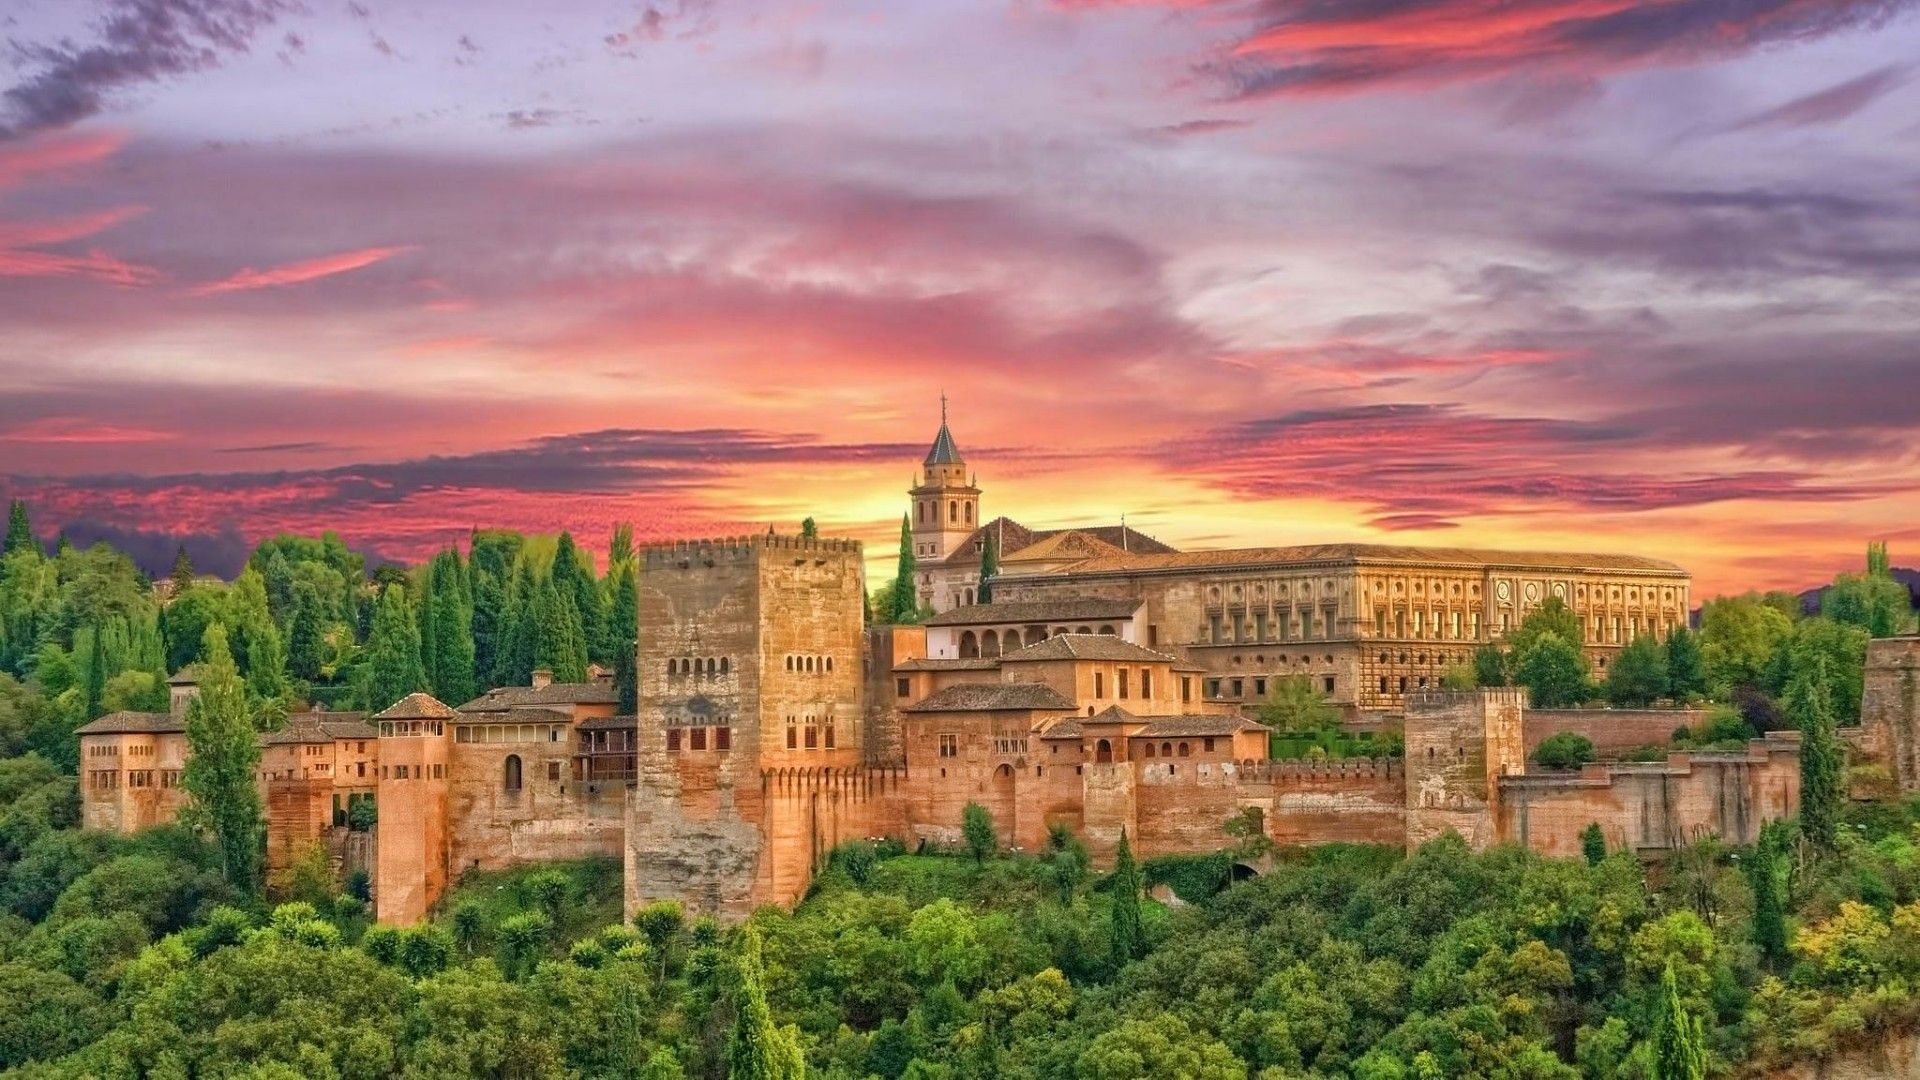
\includegraphics[width=\paperwidth,height=\paperheight,keepaspectratio]{images/granada.jpg}}
}

% Inicio del documento
\begin{document}

% Portada
\maketitle
\thispagestyle{empty}

\begin{center}
    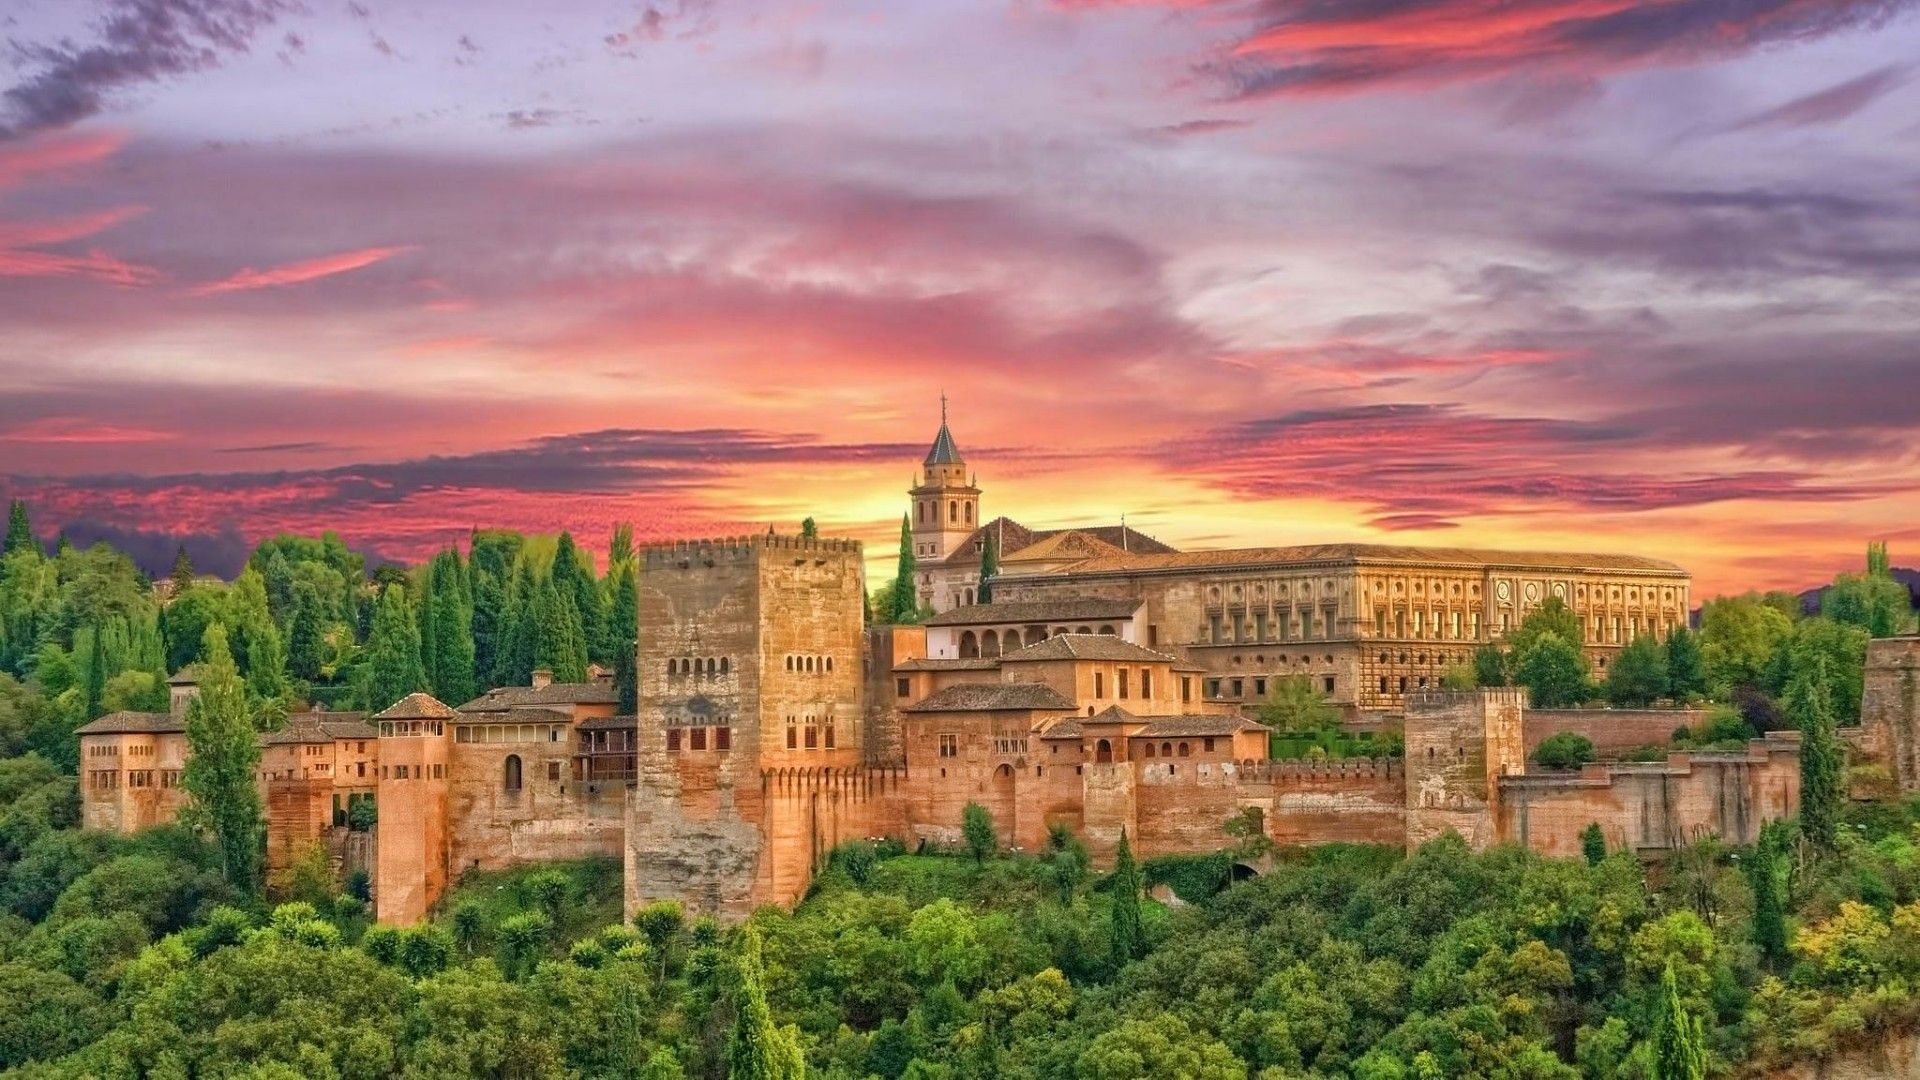
\includegraphics[width=\textwidth,height=0.4\textheight,keepaspectratio]{images/granada.jpg} \\ % Añade tu imagen de fondo
    \vfill
\end{center}

\newpage

% Índice (opcional)
\tableofcontents
\newpage

\begin{tcolorbox}[colback=red!5!white,colframe=red!75!black]
    \textit{Nota: En la resolución de estos ejercicios se sigue una metodología distinta a la teoría para algunos casos. }
    
\end{tcolorbox}

\section{Ejercicio 91}
\subsection{Enunciado}
Dado el conjunto de tareas periódicas y sus atributos temporales que se indica en la tabla de aquí abajo, determinar si se puede planificar el conjunto de dichas tareas utilizando un esquema de planificación basado en planificación cíclica. Diseña el plan cíclico determinando el marco secundario, y el entrelazamiento de las tareas sobre un cronograma.

\begin{table}[H]
\centering
\begin{tabular}{|c|c|c|c|}
\hline
\textbf{Tarea} & \textbf{Ci} & \textbf{Ti} & \textbf{Di} \\ \hline
T1 & 10 & 40 & 40 \\ \hline
T2 & 18 & 50 & 50 \\ \hline
T3 & 10 & 200 & 200 \\ \hline
T4 & 20 & 200 & 200 \\ \hline
\end{tabular}
\caption{Conjunto de tareas periódicas y sus atributos temporales}
\end{table}

\subsection{Solución}

\begin{tcolorbox}[colback=gray!5!white,colframe=gray!75!black]
    \textit{Nota: El código proporcionado en el enunciado se accede pinchando }\href{https://github.com/ElblogdeIsmael/ElblogdeIsmael.github.io/blob/main/Asignaturas/Tercer%20A%C3%B1o/SCD/Practicas/Practicas_Resueltas/Practica4/scd-p4-fuentes/SOLUCION_ACTIVIDAD_CLASE/ejecutivo2.cpp}{\textit{aquí}}.
\end{tcolorbox}

Para resolver este ejercicio aparte de poseer los conceptos teóricos necesarios de las diapositivas, vamos a servirnos de la metodología de resolución aprendida en prácticas. Este ejercicio al ser el primero será más \textit{didáctico} que el resto.

En base a este tabla:

\begin{table}[H]
    \centering
    \begin{tabular}{|c|c|c|c|}
    \hline
    \textbf{Tarea} & \textbf{Ci} & \textbf{Ti} & \textbf{Di} \\ \hline
    T1 & 10 & 40 & 40 \\ \hline
    T2 & 18 & 50 & 50 \\ \hline
    T3 & 10 & 200 & 200 \\ \hline
    T4 & 20 & 200 & 200 \\ \hline
    \end{tabular}
    \caption{Conjunto de tareas periódicas y sus atributos temporales}
\end{table}

Podemos afirmar que \[D_i = T_i \] (Para hacerlo mas similar al cpp\footnote{Proporcionado en el enlace del inicio de esta sección.}),  por lo que podemos eliminar esa columna y quedarnos con:

\begin{table}[H]
    \centering
    \begin{tabular}{|c|c|c|}
    \hline
    \textbf{Tarea} & \textbf{Ci} & \textbf{Ti} \\ \hline
    T1 & 10 & 40 \\ \hline
    T2 & 18 & 50 \\ \hline
    T3 & 10 & 200 \\ \hline
    T4 & 20 & 200 \\ \hline
    \end{tabular}
    \caption{Conjunto de tareas periódicas y sus atributos temporales}
\end{table}

Tenemos que el ciclo principal dura $T_m = mcm(T_i)\,\forall \, i 0,\ldots, 4 = 200$, de manera que nuestro ciclo secundario debe de cumplir:
\begin{enumerate}
    \item $\max(C_i) \leq T_s \leq \min(D_i)$
    \item $T_s$ divide a $T_m$, siendo el resultado $\in \mathbb{Z}$
    \item $T_s$ será un divisor del período del ciclo principal, que en este caso es 200, es decir, debe de existir un entero $K$, tal que $T_m = k \times T_S$
\end{enumerate}

En base a esto vamos a optar por escoger que el ciclo secundario debe de durar $T_s=20ms$.

Entonces, las veces que se debe de ejecutar cada tarea es:
\begin{itemize}
    \item Tarea 1 $\rightarrow$ $\frac{200}{40} = 5$ veces con un tiempo de cómputo de 10. El tiempo de cómputo máximo calculado como la sumatoria de todos los que se ejecutan en ese instante no debe de sobrepasar 20. 
    \item Tarea 2 $\rightarrow$ $\frac{200}{50} = 4$ veces con un tiempo de cómputo de 18.
    \item Tarea 3 $\rightarrow$ $\frac{200}{25} = 8$ veces con un tiempo de cómputo de 10.
    \item Tarea 4 $\rightarrow$ $\frac{200}{100} = 2$ veces con un tiempo de cómputo de 20.
\end{itemize}


Podemos afirmar que si es planificable y el cronograma quedaría de la siguiente manera:



\subsubsection{Cronograma}



\begin{table}[H]
    \centering
    \begin{tabular}{|p{1.6cm}|p{1.2cm}|p{1.2cm}|p{1.2cm}|p{1.2cm}|p{1.2cm}|p{1.2cm}|p{1.2cm}|p{1.2cm}|p{1.2cm}|p{1.2cm}|}
    \hline
    \textbf{Tiempo (ms)} & 0-20 & 20-40 & 40-60 & 60-80 & 80-100 & 100-120 & 120-140 & 140-160 & 160-180 & 180-200 \\ \hline
    \textbf{T1} & - & X & - & X & - & 1 & - & 1 & - & X \\ \hline
    \textbf{T2} & X & - & X & - & X & - & X & - & - & - \\ \hline
    \textbf{T3} & - & X & - & - & - & - & - & - & - & - \\ \hline
    \textbf{T4} & - & - & - & - & - & - & - & - & X & - \\ \hline
    \textbf{Cómputo (ms)} & 18 & 20 & 18 & 10 & 18 & 10 & 18 & 10 & 20 & 10 \\ \hline
    \end{tabular}
    \caption{Cronograma de ejecución de las tareas}
\end{table}
    
\subsubsection{Implementación en pseudo-código}

\begin{lstlisting}[style=customcpp, caption={Implementación en C++ del planificador cíclico}]

    Ts := duración del ciclo secundario;
    ini_sec := instante de inicio del ciclo secundario;

    while (true) { // ciclo principal
        for (desde i := 1 hasta 10) { // 10 porque son las fases del ciclo secundario en base a nuestro cronograma

            inicio_iteracion := instante actual;

            switch(i) {
                case 1:
                    Tarea1();
                    Tarea2();
                    break;

                case 2:
                    Tarea1();
                    break;

                case 3:
                    Tarea3();
                    break;

                case 4:
                    Tarea1();
                    Tarea2();
                    break;

                case 5:
                    Tarea1();
                    break;

                case 6:
                    Tarea2();
                    break;

                case 7:
                    Tarea1();
                    Tarea3();
                    break;

                case 8:
                    Tarea1();
                    Tarea2();
                    break;

                case 9:
                    Tarea1();
                    break;

                case 10:
                    Tarea4();
                    break;
            }

            ini_sec += Ts; // siguiente instante
            sleep_until(ini_sec); // esperar hasta el siguiente ciclo secundario
            fin_iteracion := instante actual; // medir retraso
            retraso := fin_iteracion - ini_sec; // calcular retraso
        }
    }
\end{lstlisting}



% \subsection{Solución}

% \begin{tcolorbox}[colback=gray!5!white,colframe=blue!75!black]
%     \textit{En este ejercicio al ser el primero se proporcionarán 3 soluciones válidas, después se continuará con la 2 solución, la que esta basada en la teoría de la Asignatura.}
% \end{tcolorbox}

% Para determinar si el conjunto de tareas puede ser planificado utilizando un esquema de planificación cíclica, procedemos con los siguientes pasos:

% \begin{enumerate}
%     \item \textbf{Cálculo del marco secundario ($S$):}
%     \begin{itemize}
%         \item El marco secundario debe cumplir las siguientes restricciones:
%         \begin{equation}
%         \text{Mínimo común divisor} \leq S \leq \text{Mínimo periodo de las tareas}
%         \end{equation}
%         \begin{equation}
%         \frac{T_i}{S} \in \mathbb{Z}, \quad \forall i
%         \end{equation}
%         \item Aquí, el mínimo común divisor de los periodos es:
%         \[
%         \text{MCD}(40, 50, 200, 200) = 10
%         \]
%         El mínimo periodo es $40$. Por lo tanto, $S$ debe estar en el rango $10 \leq S \leq 40$.
%         \item Probamos divisores en el rango: $S = 10, 20, 40$. Elegimos el valor que satisface todas las condiciones.
%     \end{itemize}

%     \item \textbf{Diseño del plan cíclico:}
%     \begin{itemize}
%         \item Construimos un plan cíclico asignando las tareas a intervalos de tiempo de acuerdo con sus periodos y tiempos de ejecución ($C_i$). 
%         \item Aseguramos que la suma de los tiempos de ejecución de las tareas dentro de un marco no exceda $S$.
%     \end{itemize}

%     \item \textbf{Construcción del cronograma:}
%     \begin{itemize}
%         \item Basándonos en el plan cíclico, construimos un cronograma que muestre el entrelazamiento de las tareas en el tiempo.
%     \end{itemize}
% \end{enumerate}

% \subsubsection{Cálculo del marco secundario}

% El marco secundario $S$ debe cumplir:
% \[
% \text{MCD}(40, 50, 200, 200) = 10, \quad \text{y } S \leq 40.
% \]
% Probamos divisores: $S = 10, 20, 40$. Al probar, encontramos que $S = 20$ satisface todas las condiciones.

% \subsubsection{Diseño del cronograma}

% Con $S = 20$, asignamos las tareas en bloques de tiempo. El diseño del plan cíclico queda como sigue:

% \begin{verbatim}
% Marco 1: T1, T2
% Marco 2: T1
% Marco 3: T3
% Marco 4: T4
% \end{verbatim}

% \subsubsection{Visualización del cronograma}

% El cronograma resultante es:

% \begin{table}[H]
% \centering
% \begin{tabular}{|c|c|c|c|c|}
% \hline
% \textbf{Marco} & \textbf{0--20} & \textbf{20--40} & \textbf{40--60} & \textbf{60--80} \\ \hline
% \textbf{Tareas} & T1, T2 & T1 & T3 & T4 \\ \hline
% \end{tabular}
% \caption{Cronograma del plan cíclico}
% \end{table}

% Por lo tanto, el conjunto de tareas es planificable utilizando un esquema de planificación cíclica.

% \subsection{Solución basada en la teoría}

% De acuerdo con la teoría de planificación cíclica, los pasos para resolver el problema son los siguientes:

% \begin{enumerate}
%     \item \textbf{Cálculo del hiperperiodo ($T_M$):}
%     \begin{itemize}
%         \item El hiperperiodo es el mínimo común múltiplo de los periodos de las tareas ($T_i$):
%         \[
%         T_M = \text{mcm}(40, 50, 200) = 200
%         \]
%         Este valor indica la duración del ciclo principal de planificación.
%     \end{itemize}

%     \item \textbf{Determinación del marco secundario ($T_S$):}
%     \begin{itemize}
%         \item Según la teoría, el marco secundario debe cumplir:
%         \[
%         \text{máximo } C_i \leq T_S \leq \text{mínimo } D_i
%         \]
%         \[
%         T_S \text{ divide exactamente a } T_M
%         \]
%         En este caso:
%         \[
%         \max(C_i) = 20, \quad \min(D_i) = 40
%         \]
%         Probamos divisores de 200 en el rango $20 \leq T_S \leq 40$: los valores posibles son $20$ y $40$. Seleccionamos $T_S = 20$ para optimizar el ajuste.
%     \end{itemize}

%     \item \textbf{Construcción del plan cíclico:}
%     \begin{itemize}
%         \item Dividimos el hiperperiodo en $T_M / T_S = 200 / 20 = 10$ marcos secundarios.
%         \item Asignamos las tareas a cada marco respetando sus periodos y tiempos de ejecución ($C_i$).
%     \end{itemize}
% \end{enumerate}

% \subsubsection{Plan cíclico diseñado}

% El plan cíclico diseñado con $T_S = 20$ se muestra a continuación:

% \begin{table}[H]
% \centering
% \begin{tabular}{|c|c|c|c|c|}
% \hline
% \textbf{Marco} & \textbf{0--20} & \textbf{20--40} & \textbf{40--60} & \textbf{60--80} \\ \hline
% \textbf{Tareas} & T1, T2 & T1 & T3 & T4 \\ \hline
% \end{tabular}
% \caption{Cronograma parcial del plan cíclico}
% \end{table}

% El cronograma completo repite este patrón hasta completar el hiperperiodo de $200$.

% \subsubsection{Validación de la planificabilidad}

% Verificamos que cada tarea cumple su plazo de respuesta:
% \begin{itemize}
%     \item $T1$: Ejecutada cada 40 ms, dentro de su plazo $D_1 = 40$.
%     \item $T2$: Ejecutada cada 50 ms, dentro de su plazo $D_2 = 50$.
%     \item $T3$: Ejecutada cada 200 ms, dentro de su plazo $D_3 = 200$.
%     \item $T4$: Ejecutada cada 200 ms, dentro de su plazo $D_4 = 200$.
% \end{itemize}

% Por lo tanto, el sistema es planificable con el esquema de planificación cíclica.

% \subsubsection{Extra}
% En la tabla, los valores $T_i$, $D_i$, y $C_i$ corresponden a los principales atributos temporales de una tarea en sistemas de tiempo real, según la teoría explicada en tu documento. Estos son:

% \begin{itemize}
%     \item $T_i$: Periodo de la tarea
%     \begin{itemize}
%         \item Es el intervalo de tiempo entre activaciones consecutivas de la tarea.
%         \item Indica cada cuánto tiempo debe ejecutarse la tarea.
%         \item Ejemplo: Para $T_1=40$, la tarea $T_1$ debe activarse cada 40 milisegundos.
%     \end{itemize}

%     \item $D_i$: Deadline o plazo de respuesta máximo
%     \begin{itemize}
%         \item Es el tiempo límite dentro del cual la tarea debe completarse después de ser activada.
%         \item Usualmente, $D_i$ coincide con el periodo $T_i$, pero no necesariamente (puede ser menor).
%         \item Ejemplo: $D_1=40$ significa que $T_1$ debe completarse dentro de 40 milisegundos tras su activación.
%     \end{itemize}

%     \item $C_i$: Tiempo de cómputo máximo
%     \begin{itemize}
%         \item Es el tiempo máximo requerido por la tarea para completar su ejecución, bajo las peores condiciones posibles (WCET, Worst Case Execution Time).
%         \item Este valor representa el recurso temporal mínimo que necesita la tarea en cada activación.
%         \item Ejemplo: $C_1=10$ significa que $T_1$ necesita un máximo de 10 milisegundos de tiempo de procesador para completarse.
%     \end{itemize}
% \end{itemize}

% En resumen:
% \begin{itemize}
%     \item $T_i$: Cada cuánto se activa la tarea.
%     \item $D_i$: Cuándo debe haber terminado como máximo.
%     \item $C_i$: Cuánto tiempo de CPU necesita para completarse.
% \end{itemize}

% \subsection{Solución ajustada al código proporcionado}
% \begin{tcolorbox}[colback=gray!5!white,colframe=gray!75!black]
%     \textit{Nota: El código proporcionado en el enunciado se accede pinchando }\href{https://github.com/ElblogdeIsmael/ElblogdeIsmael.github.io/blob/main/Asignaturas/Tercer%20A%C3%B1o/SCD/Practicas/Practicas_Resueltas/Practica4/scd-p4-fuentes/SOLUCION_ACTIVIDAD_CLASE/ejecutivo2.cpp}{\textit{aquí}}.
% \end{tcolorbox}


% A continuación, presentamos una solución para el problema utilizando los datos del código y basándonos en los principios de planificación cíclica:
% \subsubsection{Código}
% \begin{lstlisting}[style=customcpp, caption={Solución al problema de planificación cíclica}]
% // ------------------------------------------
% // Solución al ejercicio 91 basada en planificación cíclica
% // 
% // Implementación del ejecutivo cíclico:
% // Datos de las tareas:
% // ------------
% // Ta.   T     C
% // ------------
% // T1    40    10
% // T2    50    18
% // T3    200   10
% // T4    200   20
% // ------------
% // 
% // Planificación diseñada con Ts == 20 ms:
% //  *-----------*-----------*-----------*-----------*
% //  | T1 T2     | T1        | T3        | T4        |
% //  *-----------*-----------*-----------*-----------*
% // 
% // ----------------------------------------------------

% #include <string>
% #include <iostream>
% #include <thread>
% #include <chrono>
% #include <iomanip>

% using namespace std;
% using namespace std::chrono;
% using namespace std::this_thread;

% // Tipo para duraciones en segundos y milisegundos, en coma flotante
% typedef duration<float, ratio<1, 1000>> milliseconds_f;

% // Función genérica para representar tareas
% void Tarea(const std::string &nombre, milliseconds tcomputo)
% {
%     cout << "   Comienza tarea " << nombre << " (C == " << tcomputo.count() << " ms.) ... ";
%     sleep_for(tcomputo);
%     cout << "fin." << endl;
% }

% // Tareas específicas del problema
% void Tarea1() { Tarea("T1", milliseconds(10)); }
% void Tarea2() { Tarea("T2", milliseconds(18)); }
% void Tarea3() { Tarea("T3", milliseconds(10)); }
% void Tarea4() { Tarea("T4", milliseconds(20)); }

% int main()
% {
%     // Definición del marco secundario
%     const milliseconds Ts_ms(20);

%     // Instante de inicio del ciclo principal
%     time_point<steady_clock> ini_sec = steady_clock::now();

%     while (true) // Ciclo principal
%     {
%         cout << endl
%              << "---------------------------------------" << endl
%              << "Comienza iteración del ciclo principal." << endl;

%         for (int i = 1; i <= 4; i++) // Ciclo secundario (4 iteraciones)
%         {
%             cout << endl
%                  << "Comienza iteración " << i << " del ciclo secundario." << endl;

%             time_point<steady_clock> inicio_iteracion = steady_clock::now();

%             switch (i)
%             {
%             case 1:
%                 Tarea1();
%                 Tarea2();
%                 break;
%             case 2:
%                 Tarea1();
%                 break;
%             case 3:
%                 Tarea3();
%                 break;
%             case 4:
%                 Tarea4();
%                 break;
%             }

%             // Calcular el siguiente instante de inicio
%             ini_sec += Ts_ms;

%             // Esperar hasta el siguiente ciclo secundario
%             sleep_until(ini_sec);

%             // Medir el retraso respecto al tiempo teórico esperado
%             time_point<steady_clock> fin_iteracion = steady_clock::now();
%             milliseconds_f retraso = milliseconds_f(fin_iteracion - ini_sec);
%             cout << "Retraso al final de la iteración " << i << ": " << retraso.count() << " ms." << endl;
%         }
%     }
% }

% \end{lstlisting}

% \subsubsection{Explicación}

% \paragraph{Cálculo del Marco Secundario $T_S$:}
% \begin{itemize}
%     \item Restricciones de $T_S$:
%         \begin{itemize}
%             \item $\text{máximo } C_i = 20\,\text{ms}$.
%             \item $T_S$ divide a $T_M = \text{mcm}(40, 50, 200) = 200\,\text{ms}$.
%         \end{itemize}
%     \item Elegimos $T_S = 20\,\text{ms}$.
% \end{itemize}

% \paragraph{Planificación de las Tareas:}
% \begin{itemize}
%     \item Ciclo principal con $T_M = 200\,\text{ms}$, dividido en 10 marcos secundarios de $T_S = 20\,\text{ms}$.
%     \item Asignación de las tareas:
%         \begin{itemize}
%             \item Marco 1: $T_1, T_2$
%             \item Marco 2: $T_1$
%             \item Marco 3: $T_3$
%             \item Marco 4: $T_4$
%         \end{itemize}
% \end{itemize}

% \paragraph{Conclusión:}
% \begin{itemize}
%     \item La planificación cíclica es correcta y asegura que todas las tareas cumplen sus plazos ($D_i = T_i$).
%     \item El sistema es planificable usando $T_S = 20\,\text{ms}$.
% \end{itemize}

\section{Ejercicio 92}
\subsection{Enunciado}
El siguiente conjunto de tareas periódicas se puede planificar con ejecutivos cíclicos. Determina si esto es cierto calculando el marco secundario que debería tener. Dibuja el cronograma que muestre las ocurrencias de cada tarea y su entrelazamiento. ¿Cómo se tendría que implementar? (escribe el pseudo-código de la implementación).

\begin{table}[H]
\centering
\begin{tabular}{|c|c|c|c|}
\hline
\textbf{Tarea} & \textbf{Ci} & \textbf{Ti} & \textbf{Di} \\ \hline
T1 & 2 & 6 & 6 \\ \hline
T2 & 2 & 8 & 8 \\ \hline
T3 & 3 & 12 & 12 \\ \hline
\end{tabular}
\caption{Conjunto de tareas periódicas y sus atributos temporales}
\end{table}

\subsection{Solución}
\begin{tcolorbox}[colback=gray!5!white,colframe=gray!75!black]
    \textit{Nota: Este ejercicio se resolverá siguiendo las metodologías vistas en clase y prácticas. Además, será similar a la resolución anterior del ejercicio 91.}
\end{tcolorbox}

\subsubsection{Paso 1: Verificación inicial}
Podemos observar que \(D_i = T_i\) para todas las tareas, lo que simplifica la verificación inicial. Esto significa que podemos eliminar la columna \(D_i\) y trabajar únicamente con \(C_i\) y \(T_i\):

\begin{table}[H]
\centering
\begin{tabular}{|c|c|c|}
\hline
\textbf{Tarea} & \textbf{Ci} & \textbf{Ti} \\ \hline
T1 & 2 & 6 \\ \hline
T2 & 2 & 8 \\ \hline
T3 & 3 & 12 \\ \hline
\end{tabular}
\caption{Conjunto simplificado de tareas periódicas}
\end{table}

\subsubsection{Paso 2: Cálculo del marco secundario}
El ciclo principal es el mínimo común múltiplo de los períodos \(T_i\):
\[ T_m = \text{mcm}(6, 8, 12) = 24 \text{ ms} \]

El marco secundario \(T_s\) debe cumplir:
\begin{enumerate}
    \item \(\max(C_i) \leq T_s \leq \min(D_i)\)
    \item \(T_s\) divide a \(T_m\) de manera exacta (\(T_m / T_s \in \mathbb{Z}\)).
\end{enumerate}

\textbf{Restricción 1:} \(\max(C_i) = 3 \leq T_s \leq \min(T_i) = 6\).

\textbf{Restricción 2:} \(T_s\) debe dividir a \(T_m = 24\). Los divisores de 24 dentro del rango permitido son:\[T_s = 3, 4, 6\].

Escogemos \(T_s = 6\) ya que cumple con ambas restricciones.

\subsubsection{Paso 3: Cronograma}
Dado \(T_s = 6\), construimos el cronograma:

\begin{table}[H]
\centering
\begin{tabular}{|c|c|c|c|c|c|c|}
\hline
\textbf{Tiempo (ms)} & 0-6 & 6-12 & 12-18 & 18-24 \\ \hline
\textbf{T1} & X & X & X & X \\
\textbf{T2} & - & X & - & X \\
\textbf{T3} & X & - & X & - \\
\hline
\end{tabular}
\caption{Cronograma de ejecución de las tareas}
\end{table}


\textit{Podemos afirmar que no es planificabgle, debido a que no se puede ejecutar correctamente, ya que la tarea 2 debe de ejecutarse 3 veces, pero no puede.}
% \subsubsection{Paso 4: Implementación en pseudo-código}

% \begin{lstlisting}[style = customcpp, caption = {Implementación en C++ del planificador cíclico}]

%     Ts := duración del ciclo secundario;
%     ini_sec := instante de inicio del ciclo secundario;
%     while(true){ //ciclo principal
%         for(desde i hasta 4){ // 4 porque son las fases del ciclo secundario en base a nuestro cronograma

%             inicio_iteracion := instante actual;

%             switch(i){
%                 case 1:
%                     Tarea1();
%                     break;
%                 case 2:
%                     Tarea1();
%                     Tarea2();
%                     break;
%                 case 3:
%                     Tarea1();
%                     Tarea3();
%                     break;
%                 case 4:
%                     Tarea1();
%                     Tarea2();
%                     break;
                
%             }

%             ini_sec += Ts; //siguiente instante
%             sleep_until(ini_sec); //esperar hasta el siguiente ciclo secundario
%             fin_iteracion := instante actual; //medir retraso
%             retraso := fin_iteracion - ini_sec; //calcular retraso

%         }
%     }
% \end{lstlisting}

% Con esto confirmamos que el conjunto de tareas se puede planificar con un esquema de planificación cíclica utilizando \(T_s = 6\).

\section{Ejercicio 93}
\subsection{Enunciado}
Comprobar si el conjunto de procesos periódicos que se muestra en la siguiente tabla es planificable con el algoritmo RMS utilizando el test basado en el factor de utilización del tiempo del procesador. Si el test no se cumple, ¿debemos descartar que el sistema sea planificable?

\begin{table}[H]
\centering
\begin{tabular}{|c|c|c|}
\hline
\textbf{Tarea} & \textbf{Ci} & \textbf{Ti} \\ \hline
T1 & 9 & 30 \\ \hline
T2 & 10 & 40 \\ \hline
T3 & 10 & 50 \\ \hline
\end{tabular}
\caption{Conjunto de procesos periódicos}
\end{table}

\subsection{Solución}
El algoritmo \textbf{Rate Monotonic Scheduling (RMS)} es un esquema de planificación de tiempo real que asigna prioridades de manera estática a tareas periódicas. Las prioridades están inversamente relacionadas con los periodos (\(T_i\)): menor periodo, mayor prioridad. Este método utiliza el factor de utilización del procesador (\(U\)) para determinar si un conjunto de tareas es planificable.

El test de planificabilidad se basa en:
\[
U = \sum_{i=1}^{N} \frac{C_i}{T_i}, \quad U \leq U_0(N) = N \cdot (2^{\frac{1}{N}} - 1)
\]

Para \(N = 3\):
\[
U_0(3) = 3 \cdot (2^{\frac{1}{3}} - 1) \approx 0.779
\]

Cálculo del factor de utilización:
\[
U = \frac{9}{30} + \frac{10}{40} + \frac{10}{50} = 0.3 + 0.25 + 0.2 = 0.75
\]

\textbf{Conclusión:} El sistema es planificable porque \(U = 0.75 \leq U_0(3) = 0.779\).

Si \(U > U_0(N)\), no podemos descartar automáticamente la planificabilidad. Deberíamos construir un cronograma utilizando un diagrama de Gantt para verificar si todas las tareas cumplen sus plazos, ya que como se afirma en la teoría no se puede afirmar nada, es solo condición suficiente.

\subsubsection{Implementación en pseudo-código}

\textit{Nota: podemos implementar el algoritmo RMS en C++ de la siguiente manera usando los módulos ya que sería seguir una lógica similar a la de teoría y prácticas de la Asignatura.}

\begin{lstlisting}[style=customcpp, caption={Implementación en C++ del algoritmo RMS}]
    // Prioridades: T1 > T2 > T3 (porque T1 tiene el menor período)
    while (true) {
        tiempo_actual := instante_actual();
        
        if (tiempo_actual % 30 == 0) {
            ejecutar(T1);
        }
        if (tiempo_actual % 40 == 0) {
            ejecutar(T2);
        }
        if (tiempo_actual % 50 == 0) {
            ejecutar(T3);
        }
        
        tiempo_siguiente := tiempo_actual + intervalo_minimo();
        sleep_until(tiempo_siguiente);
    }
\end{lstlisting}

Este código asegura que las tareas se ejecutan según sus prioridades y periodos definidos. Si necesitas el diagrama de Gantt o más detalles, avísame.

\section{Ejercicio 94}
\subsection{Enunciado}
Considérese el siguiente conjunto de tareas compuesto por tres tareas periódicas:

\begin{table}[H]
\centering
\begin{tabular}{|c|c|c|}
\hline
\textbf{Tarea} & \textbf{Ci} & \textbf{Ti} \\ \hline
T1 & 10 & 40 \\ \hline
T2 & 20 & 60 \\ \hline
T3 & 20 & 80 \\ \hline
\end{tabular}
\caption{Conjunto de tareas periódicas}
\end{table}

Comprobar la planificabilidad del conjunto de tareas con el algoritmo RMS utilizando el test basado en el factor de utilización. Calcular el hiperperiodo y construir el correspondiente cronograma.

\subsection{Solución}
\subsubsection{Cálculo del factor de utilización}
El algoritmo \textbf{Rate Monotonic Scheduling (RMS)} establece que las tareas son planificables si su factor de utilización (\(U\)) cumple:
\[
U = \sum_{i=1}^{N} \frac{C_i}{T_i} \quad \text{y} \quad U \leq U_0(N) = N \cdot (2^{\frac{1}{N}} - 1)
\]

Para \(N = 3\):
\[
U_0(3) = 3 \cdot (2^{\frac{1}{3}} - 1) \approx 0.779
\]

Calculamos \(U\):
\[
U = \frac{10}{40} + \frac{20}{60} + \frac{20}{80} = 0.25 + 0.333 + 0.25 = 0.833
\]

\textbf{Conclusión:} \(U = 0.833 > 0.779\), por lo que el conjunto de tareas no pasa el test basado en el factor de utilización. Sin embargo, esto no significa que el sistema no sea planificable. Es necesario construir el cronograma para verificarlo.

\subsubsection{Cálculo del hiperperiodo}
El hiperperiodo (\(T_m\)) es el mínimo común múltiplo (\(\text{mcm}\)) de los períodos de las tareas:
\[
T_m = \text{mcm}(40, 60, 80) = 240 \, \text{ms}
\]

\subsubsection{Cronograma}
Si intentamos hacer el cronograma vemos que no es posible debido a que en una de las fases no podemos ejecutar las 3 tareas debido a que sobrepasamos el tiempo de cómputo total y por ende, no podemos planificar este cronograma aunque cumpla el test RMS.

% El cronograma muestra las instancias de ejecución de las tareas en el intervalo \([0, T_m]\). Construimos una tabla para reflejar esto:

% \begin{table}[H]
% \centering
% \begin{tabular}{|p{1.4cm}|p{1cm}|p{1cm}|p{1cm}|p{1cm}|p{1cm}|p{1cm}|p{1cm}|p{1cm}|p{1cm}|p{1cm}|p{1 cm}|}
% \hline
% \textbf{Tiempo (ms)} & 0-10 & 10-20 & 20-30 & 30-40 & 40-60 & 60-80 & 80-100 & 100-120 & 120-140 & 140-160 & \ldots \\ \hline
% \textbf{T1} & X & - & X & - & X & - & X & - & X & - & \ldots \\ \hline
% \textbf{T2} & - & - & - & X & - & X & - & - & - & X & \ldots \\ \hline
% \textbf{T3} & - & - & - & - & - & - & X & - & - & - & \ldots \\ \hline
% \end{tabular}
% \caption{Cronograma de las tareas para \(T_m = 240\) ms}
% \end{table}

% \subsubsection{Implementación en pseudo-código}
% \begin{lstlisting}[style=customcpp, caption={Implementación en C++ del cronograma}]
%     while (true) {
%         tiempo_actual := instante_actual();

%         if (tiempo_actual % 40 == 0) {
%             ejecutar(T1);
%         }
%         if (tiempo_actual % 60 == 0) {
%             ejecutar(T2);
%         }
%         if (tiempo_actual % 80 == 0) {
%             ejecutar(T3);
%         }

%         tiempo_siguiente := tiempo_actual + intervalo_minimo();
%         sleep_until(tiempo_siguiente);
%     }
% \end{lstlisting}

% Con este análisis, verificamos que el cronograma asegura que todas las tareas cumplen sus plazos. Aunque no pasa el test de utilización, el sistema es planificable.

\section{Ejercicio 95}
\subsection{Enunciado}
Comprobar la planificabilidad y construir el cronograma de acuerdo al algoritmo de planificación RMS del siguiente conjunto de tareas periódicas:

\begin{table}[H]
\centering
\begin{tabular}{|c|c|c|}
\hline
\textbf{Tarea} & \textbf{Ci} & \textbf{Ti} \\ \hline
T1 & 20 & 60 \\ \hline
T2 & 20 & 80 \\ \hline
T3 & 20 & 120 \\ \hline
\end{tabular}
\caption{Conjunto de tareas periódicas}
\end{table}

\subsection{Solución}
El algoritmo \textbf{Rate Monotonic Scheduling (RMS)} asigna prioridades de manera estática en función del periodo (\(T_i\)): a menor periodo, mayor prioridad. Verificamos la planificabilidad utilizando el test basado en el factor de utilización del procesador.

\subsubsection{Cálculo del Factor de Utilización}
El factor de utilización se calcula como:
\[
U = \sum_{i=1}^N \frac{C_i}{T_i}
\]
Sustituyendo los valores de las tareas:
\[
U = \frac{20}{60} + \frac{20}{80} + \frac{20}{120} = 0.333 + 0.25 + 0.1667 = 0.7497
\]

El límite de utilización máxima (\(U_0(N)\)) para \(N = 3\) tareas es:
\[
U_0(3) = 3 \cdot (2^{\frac{1}{3}} - 1) \approx 0.779
\]

\textbf{Conclusión:} Como \(U = 0.7497 \leq U_0(3) = 0.779\), el conjunto de tareas es planificable según RMS.

\subsubsection{Cálculo del Hiperperiodo}
El hiperperiodo (\(T_m\)) es el \textbf{mínimo común múltiplo (mcm)} de los períodos de las tareas:
\[
T_m = \text{mcm}(60, 80, 120) = 240 \, \text{ms}
\]

\subsubsection{Cronograma}
El cronograma se construye considerando las instancias de activación de cada tarea en el intervalo \([0, T_m]\), donde cada tarea \(T_i\) se activa cada \(T_i\) ms y tiene un tiempo de ejecución de \(C_i\) ms.

% \begin{table}[H]
% \centering
% \begin{tabular}{|c|c|c|c|c|c|c|c|}
% \hline
% \textbf{Tiempo (ms)} & 0-20 & 20-40 & 40-60 & 60-80 & 80-100 & 100-120 & \ldots \\ \hline
% \textbf{T1} & X & - & X & - & X & - & \ldots \\ \hline
% \textbf{T2} & - & - & - & X & - & X & \ldots \\ \hline
% \textbf{T3} & - & - & - & - & - & - & \ldots \\ \hline
% \end{tabular}
% \caption{Cronograma de las tareas periódicas para \(T_m = 240\) ms}
% \end{table}
Si se puede planificar, la manera de desarollar el cronograma es similar a las realizadas anteriormente.

\textbf{Nota:} Si se requiere el diagrama de Gantt detallado, puede construirse para el hiperperiodo calculado.

\subsubsection{Implementación en Pseudo-Código}
% \begin{lstlisting}[style=customcpp, caption={Implementación en C++ del cronograma}]
%     while (true) {
%         tiempo_actual := instante_actual();

%         if (tiempo_actual % 60 == 0) {
%             ejecutar(T1);
%         }
%         if (tiempo_actual % 80 == 0) {
%             ejecutar(T2);
%         }
%         if (tiempo_actual % 120 == 0) {
%             ejecutar(T3);
%         }

%         tiempo_siguiente := tiempo_actual + intervalo_minimo();
%         sleep_until(tiempo_siguiente);
%     }
% \end{lstlisting}

En cuanto a la implementación pasa de igual manera.

Con este análisis, concluimos que el conjunto de tareas es planificable y el cronograma asegura el cumplimiento de los plazos.












%---------------------------------------------------------------------------CORREGIR----------------------------------







\section{Ejercicio 96}
\subsection{Enunciado}
Determinar si el siguiente conjunto de tareas puede planificarse con la política de planificación RMS y con la política EDF, utilizando los tests de planificabilidad adecuados para cada uno de los dos casos. Comprobar también la planificabilidad construyendo los cronogramas para ambas políticas.

\begin{table}[H]
\centering
\begin{tabular}{|c|c|c|}
\hline
\textbf{Tarea} & \textbf{Ci} & \textbf{Ti} \\ \hline
T1 & 1 & 5 \\ \hline
T2 & 1 & 10 \\ \hline
T3 & 2 & 20 \\ \hline
T4 & 10 & 20 \\ \hline
T5 & 7 & 100 \\ \hline
\end{tabular}
\caption{Conjunto de tareas periódicas}
\end{table}

\subsection{Solución}
\subsubsection{Planificación con RMS}
El algoritmo \textbf{Rate Monotonic Scheduling (RMS)} asigna prioridades de manera estática en función del periodo (\(T_i\)): a menor periodo, mayor prioridad. Verificamos la planificabilidad utilizando el test basado en el factor de utilización del procesador.

\paragraph{Test de Planificabilidad RMS}
El factor de utilización del procesador se calcula como:
\[
U = \sum_{i=1}^N \frac{C_i}{T_i}
\]

Sustituyendo los valores de las tareas:
\[
U = \frac{1}{5} + \frac{1}{10} + \frac{2}{20} + \frac{10}{20} + \frac{7}{100} = 0.2 + 0.1 + 0.1 + 0.5 + 0.07 = 0.97
\]

El límite de utilización máxima para \(N = 5\) tareas es:
\[
U_0(5) = 5 \cdot (2^{\frac{1}{5}} - 1) \approx 0.743
\]

\textbf{Conclusión:} Como \(U = 0.97 > 0.743\), el sistema \textbf{no pasa el test RMS}. Esto indica que no podemos garantizar la planificabilidad mediante este test.

\paragraph{Construcción del Cronograma RMS}
Para comprobar la planificabilidad con RMS, construimos el cronograma hasta el hiperperiodo (\(T_m\)), que es el \textbf{mcm} de los periodos:
\[
T_m = \text{mcm}(5, 10, 20, 100) = 100 \, \text{ms}
\]

\begin{table}[H]
\centering
\begin{tabular}{|c|c|c|c|c|c|c|}
\hline
\textbf{Tiempo (ms)} & 0-1 & 1-2 & 2-3 & 3-4 & 4-5 & \ldots \\ \hline
\textbf{T1} & X & - & X & - & X & \ldots \\ \hline
\textbf{T2} & - & - & - & - & X & \ldots \\ \hline
\textbf{T3} & - & - & - & X & - & \ldots \\ \hline
\textbf{T4} & - & X & X & X & X & \ldots \\ \hline
\textbf{T5} & - & - & - & - & - & \ldots \\ \hline
\end{tabular}
\caption{Cronograma RMS para \(T_m = 100\) ms}
\end{table}

Si las tareas cumplen sus plazos en \(T_m\), el sistema es planificable con RMS.


\subsubsection{Planificación con EDF}
El algoritmo \textbf{Earliest Deadline First (EDF)} asigna prioridades dinámicamente según los plazos de respuesta (\(d_i\)): a menor plazo restante, mayor prioridad. Este método utiliza el segundo test de planificabilidad de Liu y Layland:
\[
U = \sum_{i=1}^N \frac{C_i}{T_i} \quad \text{y} \quad U \leq 1
\]

\paragraph{Test de Planificabilidad EDF}
Sustituyendo los valores de las tareas:
\[
U = \frac{1}{5} + \frac{1}{10} + \frac{2}{20} + \frac{10}{20} + \frac{7}{100} = 0.97
\]

Dado que \(U = 0.97 \leq 1\), el sistema pasa el test EDF.

\paragraph{Construcción del Cronograma EDF}
Para comprobar la planificabilidad, construimos el cronograma dinámico, priorizando las tareas con menor plazo restante, hasta \(T_m = 100\).

\begin{table}[H]
\centering
\begin{tabular}{|c|c|c|c|c|c|c|}
\hline
\textbf{Tiempo (ms)} & 0-1 & 1-2 & 2-3 & 3-4 & 4-5 & \ldots \\ \hline
\textbf{T1} & X & - & X & - & X & \ldots \\ \hline
\textbf{T2} & - & - & - & - & X & \ldots \\ \hline
\textbf{T4} & - & X & X & X & X & \ldots \\ \hline
\textbf{T3} & - & - & - & X & - & \ldots \\ \hline
\textbf{T5} & - & - & - & - & - & \ldots \\ \hline
\end{tabular}
\caption{Cronograma EDF para \(T_m = 100\) ms}
\end{table}



\subsubsection{Explicación del Algoritmo EDF}
El algoritmo EDF asigna prioridades dinámicas a las tareas en función del tiempo restante hasta su plazo de respuesta absoluto (\(d_i\)). Cuando una tarea se activa, se compara su plazo con el de las demás tareas en cola de ejecución, ejecutándose aquella que tenga el plazo más cercano a expirar. EDF es óptimo para tareas periódicas y aperiódicas si \(U \leq 1\).

Ventajas del EDF:
\begin{itemize}
    \item Mayor utilización del procesador, alcanzando hasta \(U = 1\).
    \item Planificabilidad dinámica para sistemas con alta carga de tareas.
\end{itemize}

\textbf{Nota:} A pesar de pasar el test EDF, el cronograma final debe verificarse para confirmar que todas las tareas cumplen sus plazos.



\section{Ejercicio 97}
\subsection{Enunciado}
Determinar razonadamente si el siguiente conjunto de tareas puede planificarse en un sistema monoprocesador utilizando:
\begin{itemize}
    \item Un \textbf{ejecutivo cíclico}.
    \item Algún algoritmo basado en \textbf{prioridades estáticas} o \textbf{dinámicas}.
\end{itemize}

\begin{table}[H]
\centering
\begin{tabular}{|c|c|c|}
\hline
\textbf{Tarea} & \textbf{Ci} & \textbf{Ti} \\ \hline
T1 & 1 & 5 \\ \hline
T2 & 1 & 10 \\ \hline
T3 & 2 & 10 \\ \hline
T4 & 11 & 20 \\ \hline
T5 & 5 & 100 \\ \hline
\end{tabular}
\caption{Conjunto de tareas periódicas}
\end{table}

\subsection{Solución}
\subsubsection{Planificación mediante un Ejecutivo Cíclico}
El \textbf{ejecutivo cíclico} requiere que las tareas se asignen en ciclos secundarios, garantizando que todas se ejecuten dentro del hiperperiodo. Para que sea planificable:
\[
\text{TM} = \text{mcm}(5, 10, 20, 100) = 100 \, \text{ms}
\]
El tamaño del ciclo secundario (\(TS\)) debe cumplir:
\[
\max(C_i) \leq TS \leq \min(T_i)
\]
En este caso:
\[
\max(C_i) = 11 \quad \text{y} \quad \min(T_i) = 5
\]
Dado que \(11 > 5\), no es posible definir un ciclo secundario que cumpla esta condición. Por lo tanto, el sistema \textbf{no puede planificarse} mediante un ejecutivo cíclico.

\subsubsection{Planificación mediante Prioridades Estáticas (RMS)}
El algoritmo \textbf{Rate Monotonic Scheduling (RMS)} asigna prioridades según los periodos (\(T_i\)): menor \(T_i\), mayor prioridad. Calculamos el factor de utilización del procesador (\(U\)):
\[
U = \sum_{i=1}^N \frac{C_i}{T_i}
\]
Sustituyendo los valores:
\[
U = \frac{1}{5} + \frac{1}{10} + \frac{2}{10} + \frac{11}{20} + \frac{5}{100} = 0.2 + 0.1 + 0.2 + 0.55 + 0.05 = 1.1
\]
El límite de utilización máxima (\(U_0(N)\)) para \(N = 5\) tareas es:
\[
U_0(5) = 5 \cdot (2^{\frac{1}{5}} - 1) \approx 0.743
\]
Dado que \(U = 1.1 > 0.743\), el sistema \textbf{no pasa el test RMS}, y no podemos garantizar su planificabilidad con prioridades estáticas.

\subsubsection{Planificación mediante Prioridades Dinámicas (EDF)}
El algoritmo \textbf{Earliest Deadline First (EDF)} asigna prioridades según los plazos de respuesta (\(d_i\)). El test de planificabilidad EDF verifica si:
\[
U = \sum_{i=1}^N \frac{C_i}{T_i} \leq 1
\]
Sustituyendo los valores:
\[
U = \frac{1}{5} + \frac{1}{10} + \frac{2}{10} + \frac{11}{20} + \frac{5}{100} = 1.1
\]
Dado que \(U = 1.1 > 1\), el sistema \textbf{no pasa el test EDF} y no es planificable con este algoritmo.

\subsubsection{Conclusión}
\begin{itemize}
    \item \textbf{Ejecutivo Cíclico:} No es posible planificar las tareas, ya que no se puede definir un ciclo secundario que cumpla las restricciones de los periodos.
    \item \textbf{Prioridades Estáticas (RMS):} El sistema no pasa el test de utilización RMS, por lo que no es posible garantizar su planificabilidad.
    \item \textbf{Prioridades Dinámicas (EDF):} Aunque EDF es más eficiente, el sistema tampoco pasa el test, ya que el factor de utilización excede \(1\).
\end{itemize}

En resumen, este conjunto de tareas \textbf{no puede planificarse} en un sistema monoprocesador utilizando ninguno de los métodos mencionados.



\section*{Ejercicios Adicionales}

\section{Ejercicio 98}
\subsection{Enunciado}
Para el conjunto de tareas cuyos datos se muestran más abajo, se pide:
\begin{enumerate}
    \item Dibujar el gráfico de ejecución y obtener el tiempo de respuesta de cada tarea.
    \item Determinar, mediante inspección del gráfico anterior, cuántas veces interfiere la tarea \(T_1\) a la tarea \(T_3\) durante un intervalo temporal dado por el tiempo de respuesta de esta última tarea.
    \item Hacer lo mismo que en (b), pero para las tareas \(T_1\) y \(T_2\).
\end{enumerate}

\begin{table}[H]
\centering
\begin{tabular}{|c|c|c|c|}
\hline
\textbf{Tarea} & \textbf{Ci} & \textbf{Ti} & \textbf{Di} \\ \hline
T1 & 1 & 3 & 2 \\ \hline
T2 & 3 & 6 & 5 \\ \hline
T3 & 2 & 13 & 13 \\ \hline
\end{tabular}
\caption{Conjunto de tareas periódicas}
\end{table}

\subsection{Solución}
\subsubsection{Paso 1: Cálculo del hiperperiodo y prioridades}
El hiperperiodo (\(T_m\)) es el mínimo común múltiplo de los períodos (\(T_i\)):
\[
T_m = \text{mcm}(3, 6, 13) = 78 \, \text{ms}.
\]

Asignamos las prioridades utilizando el algoritmo \textbf{Rate Monotonic Scheduling (RMS)}, donde las tareas con menor período tienen mayor prioridad. Por lo tanto, el orden de prioridad es:
\[
T_1 > T_2 > T_3.
\]

\subsubsection{Paso 2: Construcción del cronograma}
El cronograma refleja los momentos en que las tareas comienzan y terminan en el intervalo \([0, T_m = 78]\). Consideramos los tiempos de cómputo (\(C_i\)) y los períodos (\(T_i\)) de las tareas:

\begin{table}[H]
\centering
\begin{tabular}{|c|c|c|c|c|c|c|c|c|c|}
\hline
\textbf{Tiempo (ms)} & 0--1 & 1--3 & 3--4 & 4--7 & 7--9 & 9--10 & 10--11 & 12--13 & 13--15 \\ \hline
\textbf{T1} & X & -- & X & -- & X & -- & X & -- & X \\ \hline
\textbf{T2} & -- & X & -- & X & X & X & -- & -- & X \\ \hline
\textbf{T3} & -- & -- & -- & -- & -- & -- & -- & X & X \\ \hline
\end{tabular}
\caption{Cronograma de ejecución en el intervalo \([0, T_m = 78]\)}
\end{table}

\textbf{Explicación del cronograma:}
\begin{itemize}
    \item \(T_1\): Se ejecuta cada 3 ms durante \(C_1 = 1\) ms, comenzando en 0, 3, 6, etc.
    \item \(T_2\): Se ejecuta cada 6 ms durante \(C_2 = 3\) ms, comenzando en 6, 12, etc.
    \item \(T_3\): Se ejecuta cada 13 ms durante \(C_3 = 2\) ms, comenzando en 13, 26, etc.
\end{itemize}

\subsubsection{Paso 3: Cálculo de los tiempos de respuesta}
El tiempo de respuesta (\(R_i\)) de cada tarea es el intervalo desde su activación hasta la finalización de su ejecución, considerando interferencias de tareas con mayor prioridad.

\begin{enumerate}
    \item \textbf{\(T_1\):} Tiene la mayor prioridad, por lo que no sufre interferencias. Su tiempo de respuesta es:
    \[
    R_1 = C_1 = 1 \, \text{ms}.
    \]

    \item \textbf{\(T_2\):} Sufre interferencias de \(T_1\), que se ejecuta una vez durante el período de \(T_2\):
    \[
    R_2 = C_2 + \text{interferencia de } T_1 = 3 + 1 = 4 \, \text{ms}.
    \]

    \item \textbf{\(T_3\):} Sufre interferencias de \(T_1\) y \(T_2\). Durante el tiempo de respuesta de \(T_3\), \(T_1\) se ejecuta 4 veces y \(T_2\) 2 veces:
    \[
    R_3 = C_3 + 4 \cdot C_1 + 2 \cdot C_2 = 2 + 4 \cdot 1 + 2 \cdot 3 = 2 + 4 + 6 = 12 \, \text{ms}.
    \]
\end{enumerate}

\subsubsection{Paso 4: Interferencias entre tareas}
\begin{itemize}
    \item \textbf{\(T_1\) y \(T_3\):} Durante \(R_3 = 12 \, \text{ms}\), \(T_1\) se ejecuta 4 veces (en los intervalos 0-1, 3-4, 6-7, y 9-10).
    \item \textbf{\(T_1\) y \(T_2\):} Durante \(R_2 = 4 \, \text{ms}\), \(T_1\) se ejecuta 1 vez (en el intervalo 0-1).
\end{itemize}

\subsubsection{Conclusión}
\begin{itemize}
    \item Todas las tareas cumplen sus plazos límites (\(D_i\)).
    \item \(T_1\) interfiere con \(T_3\) 4 veces durante \(R_3\).
    \item \(T_1\) interfiere con \(T_2\) 1 vez durante \(R_2\).
\end{itemize}

\section{Ejercicio 99}
\subsection{Enunciado}
Verificar la planificabilidad del siguiente conjunto de tareas utilizando para ello el algoritmo del \textbf{“Primero el del Tiempo Límite más Cercano” (EDF)}.

\begin{table}[H]
\centering
\begin{tabular}{|c|c|c|}
\hline
\textbf{Tarea} & \textbf{Ci} & \textbf{Ti} \\ \hline
T1 & 1 & 4 \\ \hline
T2 & 2 & 6 \\ \hline
T3 & 3 & 8 \\ \hline
\end{tabular}
\caption{Conjunto de tareas periódicas}
\end{table}

\subsection{Solución}
El algoritmo \textbf{EDF (Earliest Deadline First)} da prioridad a la tarea con el tiempo límite más cercano en cada instante de planificación. Para determinar la planificabilidad del sistema, usamos el test del factor de utilización y verificamos los plazos.

\subsubsection{Paso 1: Cálculo del factor de utilización}
El factor de utilización del procesador se define como:
\[
U = \sum_{i=1}^{N} \frac{C_i}{T_i},
\]
donde \(C_i\) es el tiempo de cómputo y \(T_i\) es el período de la tarea.

Para este conjunto de tareas:
\[
U = \frac{1}{4} + \frac{2}{6} + \frac{3}{8} = 0.25 + 0.333 + 0.375 = 0.958.
\]

Dado que \(U \leq 1\), el sistema es potencialmente planificable.

\subsubsection{Paso 2: Construcción del cronograma}
Para verificar la planificabilidad, construimos el cronograma en el hiperperiodo (\(T_m\)) del sistema, que es el mínimo común múltiplo de los períodos:
\[
T_m = \text{mcm}(4, 6, 8) = 24 \, \text{ms}.
\]

En cada instante, seleccionamos la tarea con el tiempo límite más cercano que esté lista para ejecutarse.

\begin{table}[H]
\centering
\begin{tabular}{|c|c|c|c|c|c|c|c|c|}
\hline
\textbf{Tiempo (ms)} & 0-1 & 1-2 & 2-3 & 3-4 & 4-5 & 5-6 & 6-7 & 7-8 \\ \hline
\textbf{T1} & X & - & - & X & X & - & - & X \\ \hline
\textbf{T2} & - & X & X & - & - & X & X & - \\ \hline
\textbf{T3} & - & - & - & - & - & - & X & X \\ \hline
\end{tabular}
\caption{Cronograma de las tareas en el intervalo \([0, T_m = 24]\)}
\end{table}

\textbf{Explicación del cronograma:}
\begin{itemize}
    \item \(T_1\): Tiene un período de 4 ms y un tiempo de cómputo de 1 ms. Se ejecuta en los intervalos \(0-1\), \(4-5\), \(8-9\), etc.
    \item \(T_2\): Tiene un período de 6 ms y un tiempo de cómputo de 2 ms. Se ejecuta en los intervalos \(1-3\), \(6-8\), \(12-14\), etc.
    \item \(T_3\): Tiene un período de 8 ms y un tiempo de cómputo de 3 ms. Se ejecuta en los intervalos \(7-10\), \(15-18\), etc.
\end{itemize}

\subsubsection{Paso 3: Verificación de los plazos}
El algoritmo EDF garantiza que las tareas cumplen sus plazos si \(U \leq 1\). Además, al observar el cronograma:
\begin{itemize}
    \item \(T_1\) cumple su plazo en cada instancia.
    \item \(T_2\) cumple su plazo en cada instancia.
    \item \(T_3\) cumple su plazo en cada instancia.
\end{itemize}

\subsubsection{Conclusión}
El sistema es planificable\footnote{Se esta tomando como referencia que \(T_s = 1ms\) para la realización de los cronogramas para ver mejor la transición de lo que pasa en el tiempo real, pero lo aconsejable es hacerlo calculado el \(T_s\) como se menciona en el primer ejercicio de esta relación.} bajo el algoritmo EDF, ya que el factor de utilización es menor o igual a 1, y el cronograma demuestra que todas las tareas cumplen sus plazos.


\section{Ejercicio 100}
\subsection{Enunciado}
Verificar la planificabilidad utilizando el algoritmo \textbf{EDF (Earliest Deadline First)} de asignación dinámica de prioridades a las tareas y construir el diagrama de ejecución de tareas para el siguiente conjunto:

\begin{table}[H]
\centering
\begin{tabular}{|c|c|c|c|}
\hline
\textbf{Tarea} & \textbf{Ci} & \textbf{Di} & \textbf{Ti} \\ \hline
T1 & 2 & 5 & 6 \\ \hline
T2 & 2 & 4 & 8 \\ \hline
T3 & 4 & 8 & 12 \\ \hline
\end{tabular}
\caption{Conjunto de tareas periódicas}
\end{table}

\subsection{Solución}
\subsubsection{Paso 1: Test del factor de utilización}
Para verificar la planificabilidad inicial, calculamos el factor de utilización del procesador:
\[
U = \sum_{i=1}^{N} \frac{C_i}{T_i}.
\]

Para este conjunto de tareas:
\[
U = \frac{2}{6} + \frac{2}{8} + \frac{4}{12} = 0.333 + 0.25 + 0.333 = 0.916.
\]

Dado que \(U \leq 1\), el sistema es potencialmente planificable bajo el algoritmo EDF. Sin embargo, para garantizar que todas las tareas cumplen sus plazos, construimos el cronograma.

\subsubsection{Paso 2: Hiperperiodo del sistema}
El hiperperiodo (\(T_m\)) es el mínimo común múltiplo de los períodos (\(T_i\)):
\[
T_m = \text{mcm}(6, 8, 12) = 24 \, \text{ms}.
\]

\subsubsection{Paso 3: Construcción del cronograma}
Usamos el algoritmo EDF para construir el cronograma. Este algoritmo asigna prioridades dinámicas según el tiempo límite más cercano (\(D_i\)) de cada tarea en el instante de planificación.

\begin{table}[H]
\centering
\begin{tabular}{|c|c|c|c|c|c|c|c|c|c|}
\hline
\textbf{Tiempo (ms)} & 0--2 & 2--4 & 4--6 & 6--8 & 8--10 & 10--12 & 12--14 & 14--16 & 16--18 \\ \hline
\textbf{T1} & X & -- & X & -- & -- & -- & X & -- & X \\ \hline
\textbf{T2} & -- & X & -- & X & -- & -- & -- & X & -- \\ \hline
\textbf{T3} & -- & -- & -- & -- & X & X & -- & -- & X \\ \hline
\end{tabular}
\caption{Cronograma de ejecución de las tareas en el intervalo \([0, T_m = 24]\)}
\end{table}

\textbf{Explicación del cronograma:}
\begin{itemize}
    \item \textbf{T1:} Se ejecuta durante \(C_1 = 2\) ms con un período \(T_1 = 6\) ms y un tiempo límite \(D_1 = 5\). Se activa en los intervalos 0-2, 4-6, 12-14, etc.
    \item \textbf{T2:} Se ejecuta durante \(C_2 = 2\) ms con un período \(T_2 = 8\) ms y un tiempo límite \(D_2 = 4\). Se activa en los intervalos 2-4, 6-8, 14-16, etc.
    \item \textbf{T3:} Se ejecuta durante \(C_3 = 4\) ms con un período \(T_3 = 12\) ms y un tiempo límite \(D_3 = 8\). Se activa en los intervalos 8-12, 16-20, etc.
\end{itemize}

\subsubsection{Paso 4: Verificación de los plazos}
Verificamos que cada tarea cumple su tiempo límite (\(D_i\)) observando el cronograma:
\begin{itemize}
    \item \textbf{T1:} Todas sus ejecuciones terminan antes del tiempo límite de 5 ms después de su activación.
    \item \textbf{T2:} Todas sus ejecuciones terminan antes del tiempo límite de 4 ms después de su activación.
    \item \textbf{T3:} Todas sus ejecuciones terminan antes del tiempo límite de 8 ms después de su activación.
\end{itemize}

\subsubsection{Conclusión}
El sistema es planificable bajo el algoritmo EDF, ya que:
\begin{itemize}
    \item El factor de utilización es menor o igual a 1 (\(U = 0.916 \leq 1\)).
    \item Todas las tareas cumplen sus tiempos límite (\(D_i\)).
\end{itemize}


\section{Ejercicio 101: Verificación de planificabilidad con Deadline Monotonic (DM)}
\subsection{Enunciado}
Verificar la planificabilidad del conjunto de tareas descrito en el ejercicio 100 utilizando el algoritmo del \textbf{plazo de respuesta máximo (D)} o \textbf{Deadline Monotonic (DM)}.

\subsection{Solución}
El algoritmo \textbf{DM (Deadline Monotonic)} asigna prioridades estáticas a las tareas en función de su plazo de respuesta máximo (\(D_i\)): a menor \(D_i\), mayor prioridad. Evaluaremos si el conjunto de tareas es planificable bajo este esquema.

\subsubsection{Paso 1: Conjunto de tareas}
Para referencia, el conjunto de tareas es:
\begin{table}[H]
\centering
\begin{tabular}{|c|c|c|c|}
\hline
\textbf{Tarea} & \textbf{Ci} & \textbf{Di} & \textbf{Ti} \\ \hline
T1 & 2 & 5 & 6 \\ \hline
T2 & 2 & 4 & 8 \\ \hline
T3 & 4 & 8 & 12 \\ \hline
\end{tabular}
\caption{Conjunto de tareas periódicas}
\end{table}

\subsubsection{Paso 2: Cálculo del tiempo de respuesta (\(R_i\))}
Para determinar si las tareas son planificables, calculamos el tiempo de respuesta (\(R_i\)) para cada tarea mediante la fórmula iterativa:
\[
R_i^{(k+1)} = C_i + \sum_{j=1}^{i-1} \left\lceil \frac{R_i^{(k)}}{T_j} \right\rceil C_j
\]
\textbf{Criterio de planificabilidad:} Si \(R_i \leq D_i\) para todas las tareas, el sistema es planificable.

\paragraph{Tarea T1 (\(D_1 = 5\)):}
\[
R_1 = C_1 = 2
\]
Como \(R_1 = 2 \leq D_1 = 5\), la tarea \(T_1\) es planificable.

\paragraph{Tarea T2 (\(D_2 = 4\)):}
Iteramos el cálculo:
\[
R_2^{(0)} = C_2 = 2
\]
\[
R_2^{(1)} = C_2 + \left\lceil \frac{R_2^{(0)}}{T_1} \right\rceil C_1 = 2 + \left\lceil \frac{2}{6} \right\rceil 2 = 2 + 2 = 4
\]
Como \(R_2 = 4 \leq D_2 = 4\), la tarea \(T_2\) es planificable.

\paragraph{Tarea T3 (\(D_3 = 8\)):}
Iteramos el cálculo:
\[
R_3^{(0)} = C_3 = 4
\]
\[
R_3^{(1)} = C_3 + \left\lceil \frac{R_3^{(0)}}{T_1} \right\rceil C_1 + \left\lceil \frac{R_3^{(0)}}{T_2} \right\rceil C_2
\]
\[
R_3^{(1)} = 4 + \left\lceil \frac{4}{6} \right\rceil 2 + \left\lceil \frac{4}{8} \right\rceil 2 = 4 + 2 + 2 = 8
\]
Como \(R_3 = 8 \leq D_3 = 8\), la tarea \(T_3\) es planificable.

\subsubsection{Paso 3: Conclusión}
Todas las tareas cumplen sus plazos máximos (\(R_i \leq D_i\)):
\begin{itemize}
    \item \(R_1 = 2 \leq D_1 = 5\)
    \item \(R_2 = 4 \leq D_2 = 4\)
    \item \(R_3 = 8 \leq D_3 = 8\)
\end{itemize}
Por lo tanto, el conjunto de tareas es planificable bajo el algoritmo \textbf{Deadline Monotonic (DM)}.

\section{Ejercicio 102: Análisis de afirmaciones sobre inversión de prioridad}
\subsection{Enunciado}
Indicar cuáles de las siguientes afirmaciones son correctas respecto de los algoritmos para resolver el problema de inversión de prioridad de las tareas en sistemas de tiempo real de misión crítica:

\begin{enumerate}[label=(\alph*)]
    \item Suponiendo que las tareas se planifican con el protocolo de herencia de prioridad: la prioridad heredada por una tarea sólo se mantiene mientras dicha tarea esté utilizando un recurso compartido con otra tarea más prioritaria.
    \item Con el protocolo de techo de prioridad, cuando una tarea adquiere un recurso no puede verse interrumpida, hasta que termine su ejecución, por otras tareas que se activan después que ésta y que vayan a utilizar en el futuro un recurso con límite de prioridad igual o inferior.
    \item Con el protocolo de techo de prioridad (PPP), una tarea no puede comenzar a ejecutarse si no están libres todos los recursos que va a utilizar durante su primer ciclo.
    \item Si consideramos una tarea periódica que utilice el protocolo de techo de prioridad inmediato para cambiar su prioridad dinámica cuando accede a recursos, siempre se cumplirá que dicha tarea no puede ser interrumpida por otra menos prioritaria que ella.
    \item Con el protocolo de techo de prioridad las tareas más prioritarias del sistema pueden ser interrumpidas durante cada ciclo de su ejecución como máximo 1 vez cuando acceden a recursos que comparten con otras tareas menos prioritarias.
    \item El protocolo de techo de prioridad original producirá siempre tiempos de respuesta menores para las tareas que el algoritmo de herencia de prioridad.
\end{enumerate}

\subsection{Solución}
\subsubsection{Análisis de cada afirmación}
\begin{itemize}
    \item \textbf{(a)} \textit{Correcta.} 
    Según el protocolo de herencia de prioridad, una tarea que bloquea a otra más prioritaria hereda su prioridad mientras esté usando el recurso compartido. Al liberar el recurso, la tarea vuelve a su prioridad original.

    \item \textbf{(b)} \textit{Incorrecta.} 
    El protocolo de techo de prioridad asegura que una tarea puede ser interrumpida por otra más prioritaria, incluso si la nueva tarea no accede inmediatamente a un recurso con un techo de prioridad igual o inferior.

    \item \textbf{(c)} \textit{Incorrecta.} 
    Con el protocolo de techo de prioridad, una tarea puede comenzar a ejecutarse incluso si otros recursos que usará más adelante no están libres en ese momento.

    \item \textbf{(d)} \textit{Incorrecta.} 
    Con el protocolo de techo de prioridad inmediato, una tarea puede ser interrumpida por otra tarea que herede una prioridad más alta al acceder a un recurso compartido.

    \item \textbf{(e)} \textit{Correcta.} 
    Con el protocolo de techo de prioridad, una tarea puede ser bloqueada como máximo una vez por otras tareas menos prioritarias durante cada ciclo de su ejecución.

    \item \textbf{(f)} \textit{Incorrecta.} 
    El protocolo de techo de prioridad no garantiza tiempos de respuesta menores en todos los casos respecto al protocolo de herencia de prioridad. Dependerá de la configuración específica del sistema y las tareas.
\end{itemize}

\subsubsection{Conclusión}
Las afirmaciones \textbf{(a)} y \textbf{(e)} son \textbf{correctas}, mientras que las restantes son \textbf{incorrectas}.

\section{Ejercicio 103: Utilización máxima del procesador para un Servidor Esporádico}
\subsection{Enunciado}
Calcular la utilización máxima del procesador que se puede asignar al Servidor Esporádico para garantizar la planificabilidad del siguiente conjunto de tareas periódicas utilizando el algoritmo \textbf{Rate Monotonic (RM)}.

\begin{table}[H]
\centering
\begin{tabular}{|c|c|c|}
\hline
\textbf{Tarea} & \textbf{Ci} & \textbf{Ti} \\ \hline
$\tau_1$ & 1 & 5 \\ \hline
$\tau_2$ & 2 & 8 \\ \hline
\end{tabular}
\caption{Conjunto de tareas periódicas}
\end{table}

\subsection{Solución}
\subsubsection{Paso 1: Utilización del procesador por las tareas periódicas}
La utilización del procesador por las tareas periódicas (\(U_p\)) se calcula como:
\[
U_p = \sum_{i=1}^{N} \frac{C_i}{T_i}
\]

Sustituyendo los valores de las tareas:
\[
U_p = \frac{1}{5} + \frac{2}{8} = 0.2 + 0.25 = 0.45
\]

\subsubsection{Paso 2: Límite de utilización máxima para RM}
El límite de utilización máxima (\(U_{max}\)) para \(N = 3\) tareas (las dos tareas periódicas más el Servidor Esporádico) es:
\[
U_{max}(3) = 3 \cdot (2^{\frac{1}{3}} - 1) \approx 0.779
\]

\subsubsection{Paso 3: Utilización restante para el Servidor Esporádico}
La utilización máxima que puede asignarse al Servidor Esporádico (\(U_s\)) es:
\[
U_s = U_{max}(3) - U_p
\]

Sustituyendo los valores:
\[
U_s = 0.779 - 0.45 = 0.329
\]

\subsection{Conclusión}
La utilización máxima del procesador que se puede asignar al Servidor Esporádico para garantizar la planificabilidad del conjunto de tareas periódicas utilizando RM es:
\[
\boxed{U_s = 0.329}
\]
\section{Ejercicio 104: Utilización máxima del procesador para un Servidor Diferido (SD)}
\subsection{Enunciado}
Calcular la utilización máxima del procesador que puede ser asignada al Servidor Diferido (SD) para garantizar la planificabilidad del conjunto de tareas periódicas dado en el ejercicio 103 anterior.

\begin{table}[H]
\centering
\begin{tabular}{|c|c|c|}
\hline
\textbf{Tarea} & \textbf{Ci} & \textbf{Ti} \\ \hline
$\tau_1$ & 1 & 5 \\ \hline
$\tau_2$ & 2 & 8 \\ \hline
\end{tabular}
\caption{Conjunto de tareas periódicas}
\end{table}

\subsection{Solución}
\subsubsection{Paso 1: Fórmula para el límite de utilización máxima}
Para un Servidor Diferido (SD), la utilización máxima del procesador se calcula utilizando la fórmula de límite superior de utilización para \(N\) tareas periódicas y el servidor:
\[
U_{mls} = U_s + N \cdot \left( \left( \frac{U_s + 2}{2U_s + 1} \right)^{\frac{1}{N}} - 1 \right)
\]

Donde:
\begin{itemize}
    \item \(U_s\): Utilización asignada al servidor.
    \item \(N\): Número de tareas periódicas más el servidor (\(N = 3\)).
\end{itemize}

\subsubsection{Paso 2: Sustitución de valores}
Las tareas periódicas tienen una utilización total de:
\[
U_p = \frac{1}{5} + \frac{2}{8} = 0.45
\]

Queremos calcular el valor máximo de \(U_s\) tal que \(U_{mls} \geq U_p + U_s\).

\subsubsection{Paso 3: Resolución numérica}
Sustituyendo \(U_p = 0.45\) y \(N = 3\) en la fórmula, debemos resolver:
\[
0.45 + U_s \leq U_s + 3 \cdot \left( \left( \frac{U_s + 2}{2U_s + 1} \right)^{\frac{1}{3}} - 1 \right)
\]

Resolviendo numéricamente (por iteración o métodos de aproximación), obtenemos:
\[
U_s \approx 0.204
\]

\subsection{Conclusión}
La utilización máxima del procesador que puede ser asignada al Servidor Diferido (SD) para garantizar la planificabilidad del conjunto de tareas periódicas es:
\[
\boxed{U_s \approx 0.204}
\]

\section{Ejercicio 105: Planificación de tareas aperiódicas con Servidor Diferido (SD)}
\subsection{Enunciado}
Junto con las tareas periódicas que se muestran en el ejercicio 103, definir un plan para planificar las siguientes tareas aperiódicas utilizando un Servidor Diferido (SD), que posea una utilización máxima del tiempo del procesador y prioridad intermedia.

\begin{table}[H]
\centering
\begin{tabular}{|c|c|}
\hline
\textbf{Tarea Aperiódica} & \textbf{Ci} \\ \hline
$J_1$ & 2 \\ \hline
$J_2$ & 7 \\ \hline
$J_3$ & 17 \\ \hline
\end{tabular}
\caption{Tareas aperiódicas}
\end{table}

\subsection{Solución}
\subsubsection{Paso 1: Utilización máxima del SD}
Del ejercicio 104, sabemos que la utilización máxima del Servidor Diferido (SD) para garantizar la planificabilidad de las tareas periódicas es:
\[
U_s = 0.204
\]

El período del SD (\(T_s\)) se define de manera que cumpla:
\[
U_s = \frac{C_s}{T_s}
\]
Podemos elegir un valor adecuado para \(T_s\). Por simplicidad, tomamos \(T_s = 10\):
\[
C_s = U_s \cdot T_s = 0.204 \cdot 10 = 2.04 \approx 2
\]

El SD tendrá un tiempo de cómputo \(C_s = 2\) y un período \(T_s = 10\).

\subsubsection{Paso 2: Planificación de tareas periódicas y SD}
El conjunto de tareas periódicas, junto con el SD, se planificará usando el algoritmo \textbf{Rate Monotonic (RM)}. Asignamos las prioridades:
\begin{itemize}
    \item \(\tau_1\): Período \(T_1 = 5\) (mayor prioridad).
    \item \(\tau_2\): Período \(T_2 = 8\).
    \item SD: Período \(T_s = 10\) (prioridad intermedia).
\end{itemize}

\subsubsection{Paso 3: Planificación de tareas aperiódicas con el SD}
El SD atiende las tareas aperiódicas en sus ventanas de ejecución. Para \(C_s = 2\) y \(T_s = 10\), la ventana de ejecución del SD ocurre en cada intervalo de 10 ms.

Planificamos las tareas aperiódicas \(J_1\), \(J_2\) y \(J_3\) de acuerdo con su tiempo de cómputo (\(C_i\)) y en el orden de llegada:
\begin{itemize}
    \item \(J_1\): Se completa en el primer intervalo del SD (0-10 ms).
    \item \(J_2\): Su tiempo restante se ejecuta parcialmente en los intervalos del SD (10-20 ms y 20-30 ms).
    \item \(J_3\): Comienza su ejecución después de que \(J_2\) se completa, y utiliza el intervalo del SD en (30-40 ms).
\end{itemize}

\subsubsection{Paso 4: Cronograma}
El cronograma resultante es el siguiente (en ms):

\begin{table}[H]
    \centering
    \begin{tabular}{|c|c|c|c|c|c|c|}
    \hline
    \textbf{Tiempo} & 0--5 & 5--8 & 8--10 & 10--15 & 15--20 & 20--25 \\ \hline
    \textbf{\(\tau_1\)} & X & -- & X & -- & X & -- \\ \hline
    \textbf{\(\tau_2\)} & -- & X & -- & X & -- & X \\ \hline
    \textbf{SD} & \(J_1\) & -- & \(J_1\) & \(J_2\) & \(J_2\) & \(J_3\) \\ \hline
    \end{tabular}
    \caption{Cronograma de tareas periódicas y aperiódicas}
\end{table}

\subsection{Conclusión}
El Servidor Diferido garantiza que las tareas aperiódicas \(J_1\), \(J_2\) y \(J_3\) se ejecuten utilizando un tiempo de procesador máximo \(U_s = 0.204\), manteniendo la planificabilidad de las tareas periódicas bajo \textbf{Rate Monotonic (RM)}.

\section{Ejercicio 106: Planificación con Servidor Esporádico (SS)}
\subsection{Enunciado}
Resolver el problema de planificación descrito en el ejercicio 105, utilizando un \textbf{Servidor Esporádico (SS)} que tenga una utilización máxima del procesador y prioridad intermedia.

\begin{table}[H]
\centering
\begin{tabular}{|c|c|}
\hline
\textbf{Tarea Aperiódica} & \textbf{Ci} \\ \hline
$J_1$ & 2 \\ \hline
$J_2$ & 7 \\ \hline
$J_3$ & 17 \\ \hline
\end{tabular}
\caption{Tareas aperiódicas}
\end{table}

El conjunto de tareas periódicas está definido en el ejercicio 103 como:
\begin{table}[H]
\centering
\begin{tabular}{|c|c|c|}
\hline
\textbf{Tarea Periódica} & \textbf{Ci} & \textbf{Ti} \\ \hline
$\tau_1$ & 1 & 5 \\ \hline
$\tau_2$ & 2 & 8 \\ \hline
\end{tabular}
\caption{Conjunto de tareas periódicas}
\end{table}

\subsection{Solución}
\subsubsection{Paso 1: Utilización máxima del Servidor Esporádico (SS)}
Del ejercicio 103, sabemos que la utilización máxima asignada al servidor es \(U_s = 0.204\). La relación entre el tiempo de cómputo (\(C_s\)) y el período (\(T_s\)) del servidor es:
\[
U_s = \frac{C_s}{T_s}
\]
Eligiendo \(T_s = 10\), calculamos:
\[
C_s = U_s \cdot T_s = 0.204 \cdot 10 = 2.04 \approx 2
\]
El Servidor Esporádico tiene un tiempo de cómputo \(C_s = 2\) y un período \(T_s = 10\).

\subsubsection{Paso 2: Funcionamiento del Servidor Esporádico}
El Servidor Esporádico (SS) atiende tareas aperiódicas asignando tiempo de procesador según su tiempo disponible (\(C_s\)) y regenerando este tiempo en cada período (\(T_s\)). El servidor solo se activa cuando hay tareas aperiódicas pendientes en la cola de ejecución. 

A diferencia del Servidor Diferido, el SS permite reutilizar el tiempo no consumido en un período, lo que puede mejorar la latencia para las tareas aperiódicas.

\subsubsection{Paso 3: Planificación de las tareas aperiódicas}
Las tareas aperiódicas (\(J_1\), \(J_2\), \(J_3\)) se ejecutarán en orden de llegada, utilizando el tiempo asignado al SS. Asumimos los tiempos de llegada:
\begin{itemize}
    \item \(J_1\): Llega en \(t = 0\).
    \item \(J_2\): Llega en \(t = 8\).
    \item \(J_3\): Llega en \(t = 18\).
\end{itemize}

\subsubsection{Paso 4: Cronograma de ejecución}
\begin{table}[H]
\centering
\begin{tabular}{|c|c|c|c|c|c|c|}
\hline
\textbf{Tiempo (ms)} & 0--5 & 5--8 & 8--10 & 10--15 & 15--18 & 18--20 \\ \hline
\textbf{\(\tau_1\)} & X & -- & X & -- & X & -- \\ \hline
\textbf{\(\tau_2\)} & -- & X & -- & X & -- & X \\ \hline
\textbf{SS} & \(J_1\) & -- & \(J_1\) & \(J_2\) & \(J_2\) & \(J_3\) \\ \hline
\end{tabular}
\caption{Cronograma de tareas periódicas y aperiódicas utilizando el SS}
\end{table}

\textbf{Explicación del cronograma:}
\begin{itemize}
    \item En \(t = 0\), \(J_1\) comienza a ejecutarse utilizando el tiempo del SS (\(C_s = 2\)).
    \item En \(t = 8\), \(J_2\) llega y utiliza el tiempo disponible del SS en los períodos subsiguientes.
    \item En \(t = 18\), \(J_3\) comienza a ejecutarse y continúa en el siguiente intervalo del SS.
\end{itemize}

\subsection{Conclusión}
El Servidor Esporádico (\(U_s = 0.204\)) permite planificar las tareas aperiódicas sin afectar la planificabilidad de las tareas periódicas. Además, su capacidad de regeneración mejora la latencia de respuesta para las tareas aperiódicas en comparación con el Servidor Diferido.

\section{Ejercicio 107: Planificación con Servidor Diferido (DS)}
\subsection{Enunciado}
Resolver el problema de planificación descrito en el ejercicio 105, utilizando un \textbf{Servidor Diferido (DS)} que tenga una utilización máxima del procesador y prioridad intermedia.

\begin{table}[H]
\centering
\begin{tabular}{|c|c|}
\hline
\textbf{Tarea Aperiódica} & \textbf{Ci} \\ \hline
$J_1$ & 2 \\ \hline
$J_2$ & 7 \\ \hline
$J_3$ & 17 \\ \hline
\end{tabular}
\caption{Tareas aperiódicas}
\end{table}

El conjunto de tareas periódicas está definido en el ejercicio 103 como:
\begin{table}[H]
\centering
\begin{tabular}{|c|c|c|}
\hline
\textbf{Tarea Periódica} & \textbf{Ci} & \textbf{Ti} \\ \hline
$\tau_1$ & 1 & 5 \\ \hline
$\tau_2$ & 2 & 8 \\ \hline
\end{tabular}
\caption{Conjunto de tareas periódicas}
\end{table}

\subsection{Solución}
\subsubsection{Paso 1: Utilización máxima del Servidor Diferido (DS)}
La utilización del procesador del conjunto de tareas periódicas se calcula como:
\[
U_{\text{periodicas}} = \sum_{i=1}^{n} \frac{C_i}{T_i} = \frac{1}{5} + \frac{2}{8} = 0.2 + 0.25 = 0.45
\]
Para garantizar la planificabilidad del sistema con el Servidor Diferido, el total de utilización debe ser menor o igual a 1:
\[
U_{\text{total}} = U_{\text{periodicas}} + U_s \leq 1
\]
Donde \(U_s\) es la utilización asignada al servidor diferido. Resolviendo:
\[
U_s \leq 1 - U_{\text{periodicas}} = 1 - 0.45 = 0.55
\]
La relación entre el tiempo de cómputo (\(C_s\)) y el período (\(T_s\)) del servidor diferido es:
\[
U_s = \frac{C_s}{T_s}
\]
Eligiendo \(T_s = 10\), calculamos:
\[
C_s = U_s \cdot T_s = 0.55 \cdot 10 = 5.5 \approx 5
\]
Por lo tanto, el Servidor Diferido tiene \(C_s = 5\) y \(T_s = 10\).

\subsubsection{Paso 2: Funcionamiento del Servidor Diferido}
El Servidor Diferido (DS) preserva el tiempo asignado (\(C_s\)) hasta que haya tareas aperiódicas pendientes de ejecución. Cada período (\(T_s\)) el servidor recupera su tiempo de cómputo máximo (\(C_s = 5\)).  
Dado que el DS se ejecuta con prioridad intermedia, las tareas periódicas más prioritarias no se ven afectadas.

\subsubsection{Paso 3: Planificación de las tareas aperiódicas}
Las tareas aperiódicas (\(J_1\), \(J_2\), \(J_3\)) se ejecutarán utilizando el tiempo asignado al DS. Asumimos los tiempos de llegada:
\begin{itemize}
    \item \(J_1\): Llega en \(t = 0\).
    \item \(J_2\): Llega en \(t = 8\).
    \item \(J_3\): Llega en \(t = 18\).
\end{itemize}

\subsubsection{Paso 4: Cronograma de ejecución}
\begin{table}[H]
\centering
\begin{tabular}{|c|c|c|c|c|c|c|}
\hline
\textbf{Tiempo (ms)} & 0--5 & 5--8 & 8--10 & 10--15 & 15--18 & 18--20 \\ \hline
\textbf{\(\tau_1\)} & X & -- & X & -- & X & -- \\ \hline
\textbf{\(\tau_2\)} & -- & X & -- & X & -- & X \\ \hline
\textbf{DS} & \(J_1\) & -- & \(J_1\) & \(J_2\) & \(J_2\) & \(J_3\) \\ \hline
\end{tabular}
\caption{Cronograma de tareas periódicas y aperiódicas utilizando el DS}
\end{table}

\textbf{Explicación del cronograma:}
\begin{itemize}
    \item En \(t = 0\), \(J_1\) comienza a ejecutarse utilizando \(C_s = 5\).
    \item En \(t = 8\), \(J_2\) llega y utiliza el tiempo restante del DS en \(T_s = 10\).
    \item En \(t = 18\), \(J_3\) utiliza el siguiente período del DS.
\end{itemize}

\subsection{Conclusión}
El Servidor Diferido (\(U_s = 0.55\)) permite planificar las tareas aperiódicas sin afectar la planificabilidad de las tareas periódicas. Aunque el DS garantiza una latencia predecible, puede ser menos eficiente que el Servidor Esporádico en términos de reutilización del tiempo no consumido.

\section{Ejercicio 108: Planificación con Servidor Esporádico (SS)}
\subsection{Enunciado}
Utilizar un \textbf{Servidor Esporádico (SS)} con capacidad \(C_s = 2\) y período \(T_s = 6\) para planificar las siguientes tareas:

\begin{table}[H]
\centering
\begin{tabular}{|c|c|c|}
\hline
\textbf{Tarea Periódica} & \textbf{Ci} & \textbf{Ti} \\ \hline
$\tau_1$ & 1 & 4 \\ \hline
$\tau_2$ & 2 & 6 \\ \hline
\end{tabular}
\caption{Conjunto de tareas periódicas}
\end{table}

\begin{table}[H]
\centering
\begin{tabular}{|c|c|c|}
\hline
\textbf{Tarea Aperiódica} & \textbf{Ci} & \textbf{ai} \\ \hline
$J_1$ & 2 & 2 \\ \hline
$J_2$ & 5 & 1 \\ \hline
$J_3$ & 10 & 2 \\ \hline
\end{tabular}
\caption{Conjunto de tareas aperiódicas}
\end{table}

\subsection{Solución}
\subsubsection{Paso 1: Verificación de la planificabilidad de las tareas periódicas}
La utilización total del procesador por las tareas periódicas es:
\[
U_{\text{periodicas}} = \sum_{i=1}^{n} \frac{C_i}{T_i} = \frac{1}{4} + \frac{2}{6} = 0.25 + 0.333 = 0.583
\]
Con el Servidor Esporádico (\(U_s\)), la utilización total del procesador es:
\[
U_{\text{total}} = U_{\text{periodicas}} + U_s
\]
La utilización del SS se calcula como:
\[
U_s = \frac{C_s}{T_s} = \frac{2}{6} = 0.333
\]
Entonces:
\[
U_{\text{total}} = 0.583 + 0.333 = 0.916
\]
Dado que \(U_{\text{total}} < 1\), el sistema es planificable.

\subsubsection{Paso 2: Funcionamiento del Servidor Esporádico (SS)}
El SS asigna su capacidad (\(C_s = 2\)) únicamente cuando hay tareas aperiódicas en espera. Una vez consumido su tiempo, el servidor regenera su capacidad en el próximo período (\(T_s = 6\)).

\subsubsection{Paso 3: Planificación de las tareas aperiódicas}
Las tareas aperiódicas (\(J_1\), \(J_2\), \(J_3\)) se ejecutan en orden de llegada, utilizando el tiempo asignado al SS. Asumimos los tiempos de llegada (\(a_i\)):
\begin{itemize}
    \item \(J_1\): Llega en \(t = 2\).
    \item \(J_2\): Llega en \(t = 1\).
    \item \(J_3\): Llega en \(t = 2\).
\end{itemize}

\subsubsection{Paso 4: Cronograma de ejecución}
\begin{table}[H]
\centering
\begin{tabular}{|c|c|c|c|c|c|c|c|}
\hline
\textbf{Tiempo (ms)} & 0--1 & 1--2 & 2--4 & 4--6 & 6--8 & 8--10 & 10--12 \\ \hline
\textbf{\(\tau_1\)} & X & -- & X & -- & X & -- & X \\ \hline
\textbf{\(\tau_2\)} & -- & X & -- & X & -- & X & -- \\ \hline
\textbf{SS} & -- & \(J_2\) & \(J_1\) & \(J_3\) & \(J_3\) & -- & -- \\ \hline
\end{tabular}
\caption{Cronograma de tareas periódicas y aperiódicas utilizando el SS}
\end{table}

\textbf{Explicación del cronograma:}
\begin{itemize}
    \item En \(t = 1\), \(J_2\) comienza a ejecutarse con el tiempo del SS (\(C_s = 2\)).
    \item En \(t = 2\), \(J_1\) y \(J_3\) llegan. El SS prioriza \(J_1\) por orden de llegada.
    \item En \(t = 6\), el SS regenera su capacidad y continúa ejecutando \(J_3\).
\end{itemize}

\subsection{Conclusión}
El Servidor Esporádico (\(C_s = 2\), \(T_s = 6\)) permite planificar las tareas aperiódicas sin afectar la planificabilidad de las tareas periódicas. Su capacidad de regenerar tiempo no consumido optimiza el uso del procesador.




\end{document}